%%%%%%%%%%%%%%%%%%%%%%%%%%%%%%%%%%%%%%%%%
% Classicthesis Typographic Thesis
% LaTeX Template
% Version 1.3 (15/2/14)
%
% This template has been downloaded from:
% http://www.LaTeXTemplates.com
%
% Original author:
% André Miede (http://www.miede.de)
%
% License:
% CC BY-NC-SA 3.0 (http://creativecommons.org/licenses/by-nc-sa/3.0/)
%
% General Tips:
% 1) Make sure to edit the classicthesis-config.file
% 2) New enumeration (A., B., C., etc in small caps): \begin{aenumerate} \end{aenumerate}
% 3) For margin notes: \marginpar or \graffito{}
% 4) Do not use bold fonts in this style, it is designed around them
% 5) Use tables as in the examples
% 6) See classicthesis-preamble.sty for useful commands
%
%%%%%%%%%%%%%%%%%%%%%%%%%%%%%%%%%%%%%%%%%

%----------------------------------------------------------------------------------------
%	PACKAGES AND OTHER DOCUMENT CONFIGURATIONS
%----------------------------------------------------------------------------------------

\documentclass[
		twoside,openright,titlepage,numbers=noenddot,headinclude,%1headlines,
                footinclude=true,cleardoublepage=empty,
                BCOR=5mm,paper=a4,fontsize=11pt, % Binding correction, paper type and font size
               % ngerman,american, % Languages
                ]{scrreprt} 
 

                
% Includes the file which contains all the document configurations and packages - make sure to edit this file
%%%%%%%%%%%%%%%%%%%%%%%%%%%%%%%%%%%%%%%%%
% Thesis Configuration File
%
% The main lines to change in this file are in the DOCUMENT VARIABLES
% section, the rest of the file is for advanced configuration.
%
%%%%%%%%%%%%%%%%%%%%%%%%%%%%%%%%%%%%%%%%%

%----------------------------------------------------------------------------------------
%	DOCUMENT VARIABLES
%	Fill in the lines below to enter your information into the thesis template
%	Each of the commands can be cited anywhere in the thesis
%----------------------------------------------------------------------------------------


% Remove drafting to get rid of the '[ Date - classicthesis version 4.0 ]' text at the bottom of every page
\PassOptionsToPackage{eulerchapternumbers,listings,drafting, 
                    pdfspacing, 
                    %minionprospacing,
                    subfig,beramono,eulermath,parts}{classicthesis}
% \let\marginpar\oldmarginpar

% Available options: drafting parts nochapters linedheaders eulerchapternumbers beramono eulermath pdfspacing minionprospacing tocaligned dottedtoc manychapters listings floatperchapter subfig
% Adding 'dottedtoc' will make page numbers in the table of contents flushed right with dots leading to them

\newcommand{\myTitle}{Ancestral population genomics\xspace}
\newcommand{\mySubtitle}{A coalescent hidden Markov model approach to study ancestral populations and species\xspace}
\newcommand{\myDegree}{Doctor Scientiarum (Dr.Scient.)\xspace}
\newcommand{\myName}{Thomas Mailund\xspace}
%\newcommand{\myProf}{Put name here\xspace}
%\newcommand{\myOtherProf}{Put name here\xspace}
%\newcommand{\mySupervisor}{Put name here\xspace}
%\newcommand{\myFaculty}{Put data here\xspace}
\newcommand{\myDepartment}{Bioinformatics Research Centre\xspace}
\newcommand{\myUni}{Aarhus University\xspace}
\newcommand{\myLocation}{Aarhus\xspace}
\newcommand{\myTime}{December 20xx\xspace}
\newcommand{\myVersion}{version 1.0\xspace}

%----------------------------------------------------------------------------------------
%	USEFUL COMMANDS
%----------------------------------------------------------------------------------------

\newcommand{\ie}{i.\,e.}
\newcommand{\Ie}{I.\,e.}
\newcommand{\eg}{e.\,g.}
\newcommand{\Eg}{E.\,g.} 

\newcounter{dummy} % Necessary for correct hyperlinks (to index, bib, etc.)
\providecommand{\mLyX}{L\kern-.1667em\lower.25em\hbox{Y}\kern-.125emX\@}

%----------------------------------------------------------------------------------------
%	PACKAGES
%----------------------------------------------------------------------------------------


%------------------------------------------------
 
\PassOptionsToPackage{utf8}{inputenc}
\usepackage{inputenc}
\usepackage[english]{babel}

\usepackage[natbib=true,backend=bibtex,style=nature,
            url=false,hyperref=true,sorting=none]{biblatex}
\addbibresource{Bibliography}

\PassOptionsToPackage{fleqn}{amsmath} % Math environments and more by the AMS 
\usepackage{amsmath,amssymb}
 
\PassOptionsToPackage{T1}{fontenc} % T2A for cyrillics
\usepackage{fontenc}

\usepackage{xspace} % To get the spacing after macros right
\usepackage{mparhack} % To get marginpar right
\usepackage{fixltx2e} % Fixes some LaTeX stuff 

\PassOptionsToPackage{smaller}{acronym}
\usepackage{acronym} % nice macros for handling all acronyms in the thesis
%\renewcommand{\bflabel}[1]{{#1}\hfill} % Fix the list of acronyms

\PassOptionsToPackage{pdftex}{graphicx}
\usepackage{graphicx} 


%----------------------------------------------------------------------------------------
%	FLOATS: TABLES, FIGURES AND CAPTIONS SETUP
%----------------------------------------------------------------------------------------

\usepackage{tabularx} % Better tables
\setlength{\extrarowheight}{3pt} % Increase table row height
\newcommand{\tableheadline}[1]{\multicolumn{1}{c}{\spacedlowsmallcaps{#1}}}
\newcommand{\myfloatalign}{\centering} % To be used with each float for alignment
\usepackage{caption}
\captionsetup{format=hang,font=small}
\usepackage{subfig}  

%----------------------------------------------------------------------------------------
%	CODE LISTINGS SETUP
%----------------------------------------------------------------------------------------

\usepackage{listings} 
%\lstset{emph={trueIndex,root},emphstyle=\color{BlueViolet}}%\underbar} % for special keywords
\lstset{language=Python,
keywordstyle=\color{RoyalBlue},
basicstyle=\footnotesize\ttfamily,%\small\ttfamily,
commentstyle=\color{Green}\ttfamily, % Color of comments
stringstyle=\rmfamily,
numbers=left,
numberstyle=\scriptsize,
stepnumber=1, % Increment of line numbers
numbersep=5pt, % Distance of line numbers from code listing
showstringspaces=false,
breaklines=false,
%frameround=ftff, % Uncomment for rounded frame
frame=leftline, % Frame border - none/leftline/topline/bottomline/lines/single/shadowbox/L
belowcaptionskip=.75\baselineskip % Space after the "Listing #: Desciption" text and the listing box
}

%----------------------------------------------------------------------------------------
%	HYPERREFERENCES
%----------------------------------------------------------------------------------------

\PassOptionsToPackage{pdftex,hyperfootnotes=false,pdfpagelabels}{hyperref}
\usepackage{hyperref}  % backref linktocpage pagebackref
\pdfcompresslevel=9
\pdfadjustspacing=1

\hypersetup{
% Uncomment the line below to remove all links (to references, figures, tables, etc)
%draft, 
colorlinks=true, linktocpage=true, pdfstartpage=3, pdfstartview=FitV,
% Uncomment the line below if you want to have black links (e.g. for printing black and white)
%colorlinks=false, linktocpage=false, pdfborder={0 0 0}, pdfstartpage=3, pdfstartview=FitV, 
breaklinks=true, pdfpagemode=UseNone, pageanchor=true, pdfpagemode=UseOutlines,
plainpages=false, bookmarksnumbered, bookmarksopen=true, bookmarksopenlevel=1,
hypertexnames=true, pdfhighlight=/O, urlcolor=webbrown, linkcolor=RoyalBlue, citecolor=webgreen,
%------------------------------------------------
% PDF file meta-information
pdftitle={\myTitle},
pdfauthor={\textcopyright\ \myName, \myUni, \myFaculty},
pdfsubject={},
pdfkeywords={},
pdfcreator={pdfLaTeX},
pdfproducer={LaTeX with hyperref and classicthesis}
%------------------------------------------------
}   

%----------------------------------------------------------------------------------------
%	BACKREFERENCES
%----------------------------------------------------------------------------------------

\usepackage{ifthen} % Allows the user of the \ifthenelse command
\newboolean{enable-backrefs} % Variable to enable backrefs in the bibliography
\setboolean{enable-backrefs}{false} % Variable value: true or false

\newcommand{\backrefnotcitedstring}{\relax} % (Not cited.)
\newcommand{\backrefcitedsinglestring}[1]{(Cited on page~#1.)}
\newcommand{\backrefcitedmultistring}[1]{(Cited on pages~#1.)}
\ifthenelse{\boolean{enable-backrefs}} % If backrefs were enabled
{
\PassOptionsToPackage{hyperpageref}{backref}
\usepackage{backref} % to be loaded after hyperref package 
\renewcommand{\backreftwosep}{ and~} % separate 2 pages
\renewcommand{\backreflastsep}{, and~} % separate last of longer list
\renewcommand*{\backref}[1]{}  % disable standard
\renewcommand*{\backrefalt}[4]{% detailed backref
\ifcase #1 
\backrefnotcitedstring
\or
\backrefcitedsinglestring{#2}
\else
\backrefcitedmultistring{#2}
\fi}
}{\relax} 

%----------------------------------------------------------------------------------------
%	AUTOREFERENCES SETUP
%	Redefines how references in text are prefaced for different 
%	languages (e.g. "Section 1.2" or "section 1.2")
%----------------------------------------------------------------------------------------

\makeatletter
\@ifpackageloaded{babel}
{
\addto\extrasamerican{
\renewcommand*{\figureautorefname}{Figure}
\renewcommand*{\tableautorefname}{Table}
\renewcommand*{\partautorefname}{Part}
\renewcommand*{\chapterautorefname}{Chapter}
\renewcommand*{\sectionautorefname}{Section}
\renewcommand*{\subsectionautorefname}{Section}
\renewcommand*{\subsubsectionautorefname}{Section}
}
\addto\extrasngerman{
\renewcommand*{\paragraphautorefname}{Absatz}
\renewcommand*{\subparagraphautorefname}{Unterabsatz}
\renewcommand*{\footnoteautorefname}{Fu\"snote}
\renewcommand*{\FancyVerbLineautorefname}{Zeile}
\renewcommand*{\theoremautorefname}{Theorem}
\renewcommand*{\appendixautorefname}{Anhang}
\renewcommand*{\equationautorefname}{Gleichung}
\renewcommand*{\itemautorefname}{Punkt}
}
\providecommand{\subfigureautorefname}{\figureautorefname} % Fix to getting autorefs for subfigures right
}{\relax}
\makeatother

%----------------------------------------------------------------------------------------

\usepackage{classicthesis} 

%----------------------------------------------------------------------------------------
%	CHANGING TEXT AREA 
%----------------------------------------------------------------------------------------

%\linespread{1.05} % a bit more for Palatino
%\areaset[current]{312pt}{761pt} % 686 (factor 2.2) + 33 head + 42 head \the\footskip
%\setlength{\marginparwidth}{7em}%
%\setlength{\marginparsep}{2em}%

%----------------------------------------------------------------------------------------
%	USING DIFFERENT FONTS
%----------------------------------------------------------------------------------------

%\usepackage[oldstylenums]{kpfonts} % oldstyle notextcomp
%\usepackage[osf]{libertine}
%\usepackage{hfoldsty} % Computer Modern with osf
%\usepackage[light,condensed,math]{iwona}
%\renewcommand{\sfdefault}{iwona}
%\usepackage{lmodern} % <-- no osf support :-(
%\usepackage[urw-garamond]{mathdesign} <-- no osf support :-(

\usepackage{todonotes}

\usepackage[mathpazo]{flexisym}
\usepackage{breqn}


%% Macros for handling intervals in the CTMC algebrah
\newcommand{\interval}[1]{\mathbf{\big[}#1\mathbf{\big]}}
\renewcommand{\between}[2]{\ensuremath{\mathbf{(}#1\cdots#2\mathbf{)}}\,}
\newcommand{\upto}[1]{\ensuremath{\mathbf{[}0\cdots#1\mathbf{)}\,}}

%% Symbols for likelihoods
\newcommand{\G}{\ensuremath{\mathcal{G}}}
\newcommand{\A}{\ensuremath{\mathcal{A}}}
\newcommand{\T}{\ensuremath{\mathcal{T}}}
\newcommand{\U}{\ensuremath{\mathcal{U}}}
\newcommand{\B}{\ensuremath{\mathcal{B}}}
\renewcommand{\lhd}{\ensuremath{\mathbf{L}}}

\newcommand{\argmax}{\ensuremath{\operatorname*{arg\,max}}}


%% Integration
\newcommand{\intd}{\ensuremath{\mathrm{\;d}}}

%% CPN
\newcommand{\pre}{\ensuremath{\operatorname{pre}}}
\newcommand{\post}{\ensuremath{\operatorname{post}}}
\newcommand{\samples}{\ensuremath{\mathcal{S}}}
\newcommand{\populations}{\ensuremath{\mathcal{P}}}
\newcommand{\coaltrans}{\ensuremath{\mathfrak{c}}}
\newcommand{\migtrans}{\ensuremath{\mathfrak{m}}}
\newcommand{\recombtrans}{\ensuremath{\mathfrak{r}}}

%% Other...
\newcommand{\powerset}{\ensuremath{\mathfrak{Pow}}}
\newcommand{\partition}{\ensuremath{\mathfrak{Part}}}

\begin{document}

\frenchspacing % Reduces space after periods to make text more compact
\raggedbottom % Makes all pages the height of the text on that page
\selectlanguage{english} % Select your default language - e.g. american or ngerman

%\renewcommand*{\bibname}{new name} % Uncomment to change the name of the bibliography
%\setbibpreamble{} % Uncomment to include a preamble to the bibliography - some text before the reference list starts

\pagenumbering{roman} % Roman page numbering prior to the start of the thesis content (i, ii, iii, etc)
\pagestyle{plain} % Suppress headers for the pre-content pages

%----------------------------------------------------------------------------------------
%	PRE-CONTENT THESIS PAGES
%----------------------------------------------------------------------------------------

% Title Page

\begin{titlepage}

\begin{addmargin}[-1cm]{-3cm}
\begin{center}
\large

\hfill
\vfill

\begingroup
\color{Maroon}\spacedallcaps{\myTitle} \\ \bigskip % Thesis title
\endgroup

\spacedlowsmallcaps{\myName} % Your name

\vfill


\includegraphics[width=6cm]{gfx/au-segl} \\ \bigskip % Picture

\mySubtitle \\ \medskip % Thesis subtitle
%\myDegree \\
%\myDepartment \\
%\myFaculty \\
%\myUni \\ \bigskip

\myTime\ -- \myVersion % Time and version

\vfill

\end{center}
\end{addmargin}

\end{titlepage} % Main title page
% Back of the title page

\thispagestyle{empty}

\hfill

\vfill

\noindent\myName: \textit{\myTitle,} \mySubtitle, %\myDegree, 
\textcopyright\ \myTime

% You may wish to do something with the back of the title page, such as including your supervisors, location or time frame of the work. Below is an example of doing so although you may want to tweak it to your liking.

%\bigskip

%\noindent\spacedlowsmallcaps{Supervisors}: \\
%\myProf \\
%\myOtherProf \\ 
%\mySupervisor

%\medskip \\

%\noindent\spacedlowsmallcaps{Location}: \\
%\myLocation

%\medskip \\

%\noindent\spacedlowsmallcaps{Time Frame}: \\
%\myTime
 % Back of the title page
%\cleardoublepage% Dedication

\thispagestyle{empty}
\refstepcounter{dummy}

\pdfbookmark[1]{Dedication}{Dedication} % Bookmark name visible in a PDF viewer

\vspace*{3cm}

\begin{center}
\emph{Ohana} means family. \\
Family means nobody gets left behind, or forgotten. \\ \medskip
--- Lilo \& Stitch    
\end{center}

\medskip

\begin{center}
Dedicated to the loving memory of Rudolf Miede. \\ \smallskip
1939\,--\,2005
\end{center} % Dedication page

%\cleardoublepage\include{FrontBackMatter/Foreword} % Uncomment and create a Foreword.tex to include a foreword

\cleardoublepage% Abstract

\pdfbookmark[1]{Abstract}{Abstract} % Bookmark name visible in a PDF viewer

\begingroup
\let\clearpage\relax
\let\cleardoublepage\relax
\let\cleardoublepage\relax

\chapter*{Abstract} % Abstract name

\todo[inline]{Short summary of the contents\dots}

\endgroup			

\vfill % Abstract page
%\cleardoublepage% Publications - a page listing research articles written using content in the thesis

\pdfbookmark[1]{Publications}{Publications} % Bookmark name visible in a PDF viewer

\chapter*{Publications} % Publications page text

Some ideas and figures have appeared previously in the following publications:

\bigskip


\noindent Put your publications from the thesis here. The packages \texttt{multibib} or \texttt{bibtopic} etc. can be used to handle multiple different bibliographies in your document.~\todo{Do this!} % Publications from the thesis page
\cleardoublepage% Acknowledgements

\pdfbookmark[1]{Acknowledgements}{Acknowledgements} % Bookmark name visible in a PDF viewer

\bigskip

%----------------------------------------------------------------------------------------

\begingroup

\let\clearpage\relax
\let\cleardoublepage\relax
\let\cleardoublepage\relax

\chapter*{Acknowledgements} % Acknowledgements section text

\todo[inline]{Acknowledgements}

%Put your acknowledgements here.\\
%
%\noindent Many thanks to everybody who already sent me a postcard!\\
%
%\noindent Regarding the typography and other help, many thanks go to Marco Kuhlmann, Philipp Lehman, Lothar Schlesier, Jim Young, Lorenzo Pantieri and Enrico Gregorio\footnote{Members of GuIT (Gruppo Italiano Utilizzatori di \TeX\ e \LaTeX )}, J\"org Sommer, Joachim K\"ostler, Daniel Gottschlag, Denis Aydin, Paride Legovini, Steffen Prochnow, Nicolas Repp, Hinrich Harms, Roland Winkler,  and the whole \LaTeX-community for support, ideas and some great software.
%
%\bigskip
%
%\noindent\emph{Regarding \mLyX}: The \mLyX\ port was intially done by
%\emph{Nicholas Mariette} in March 2009 and continued by
%\emph{Ivo Pletikosi\'c} in 2011. Thank you very much for your work and the contributions to the original style.

\endgroup % Acknowledgements page

\pagestyle{scrheadings} % Show chapter titles as headings

\cleardoublepage% Table of Contents - List of Tables/Figures/Listings and Acronyms

\refstepcounter{dummy}

\pdfbookmark[1]{\contentsname}{tableofcontents} % Bookmark name visible in a PDF viewer

\setcounter{tocdepth}{0} % Depth of sections to include in the table of contents - currently up to subsections

\setcounter{secnumdepth}{3} % Depth of sections to number in the text itself - currently up to subsubsections

\manualmark
\markboth{\spacedlowsmallcaps{\contentsname}}{\spacedlowsmallcaps{\contentsname}}
\tableofcontents 
\automark[section]{chapter}
\renewcommand{\chaptermark}[1]{\markboth{\spacedlowsmallcaps{#1}}{\spacedlowsmallcaps{#1}}}
\renewcommand{\sectionmark}[1]{\markright{\thesection\enspace\spacedlowsmallcaps{#1}}}

\clearpage

%\begingroup 
%\let\clearpage\relax
%\let\cleardoublepage\relax
%\let\cleardoublepage\relax
%
%%----------------------------------------------------------------------------------------
%%	List of Figures
%%----------------------------------------------------------------------------------------
%
%\refstepcounter{dummy}
%%\addcontentsline{toc}{chapter}{\listfigurename} % Uncomment if you would like the list of figures to appear in the table of contents
%\pdfbookmark[1]{\listfigurename}{lof} % Bookmark name visible in a PDF viewer
%
%\listoffigures
%
%\vspace*{8ex}
%\newpage
%
%%----------------------------------------------------------------------------------------
%%	List of Tables
%%----------------------------------------------------------------------------------------
%
%\refstepcounter{dummy}
%%\addcontentsline{toc}{chapter}{\listtablename} % Uncomment if you would like the list of tables to appear in the table of contents
%\pdfbookmark[1]{\listtablename}{lot} % Bookmark name visible in a PDF viewer
%
%\listoftables
%        
%\vspace*{8ex}
%\newpage
%    
%%----------------------------------------------------------------------------------------
%%	List of Listings
%%---------------------------------------------------------------------------------------- 
%
%\refstepcounter{dummy}
%%\addcontentsline{toc}{chapter}{\lstlistlistingname} % Uncomment if you would like the list of listings to appear in the table of contents
%\pdfbookmark[1]{\lstlistlistingname}{lol} % Bookmark name visible in a PDF viewer
%
%\lstlistoflistings 
%
%\vspace*{8ex}
%\newpage
%       
%%----------------------------------------------------------------------------------------
%%	Acronyms
%%----------------------------------------------------------------------------------------
%
%\refstepcounter{dummy}
%%\addcontentsline{toc}{chapter}{Acronyms} % Uncomment if you would like the acronyms to appear in the table of contents
%\pdfbookmark[1]{Acronyms}{acronyms} % Bookmark name visible in a PDF viewer
%
%\markboth{\spacedlowsmallcaps{Acronyms}}{\spacedlowsmallcaps{Acronyms}}
%
%\chapter*{Acronyms}
%
%\begin{acronym}[UML]
%\acro{DRY}{Don't Repeat Yourself}
%\acro{API}{Application Programming Interface}
%\acro{UML}{Unified Modeling Language}
%\end{acronym}  
%                   
%\endgroup % Contents, list of figures/tables/listings and acronyms

\cleardoublepage

\pagenumbering{arabic} % Arabic page numbering for thesis content (1, 2, 3, etc)
%\setcounter{page}{90} % Uncomment to manually start the page counter at an arbitrary value (for example if you wish to count the pre-content pages in the page count)

\cleardoublepage % Avoids problems with pdfbookmark

%----------------------------------------------------------------------------------------
%	THESIS CONTENT - CHAPTERS
%----------------------------------------------------------------------------------------


\chapter{Introduction}

A central question in biology has always be how species form and how a group of interbreeding individuals can split into two or more groups and over time evolve apart and accumulate different genetic changes until individuals from different groups are no longer able to reproduce. Despite decades of research and a wealth of theoretical models, we still know very little about this process.

\section{Ancestral population genetics}

There are two ways of studying the speciation process: observing the evolution of new species in action or making inference of speciation processes that occurred in the past. The former approach certainly provides the best data to study but is only possible in a few systems where the evolution of genetic isolation is partway done and there only provides a snapshot of a single time point in that evolution. The number of systems we can study by making inference from past speciation events is much greater and by careful modelling of the process we can study the entire process of speciation.

Studying ancient speciation events requires us to do population genetics in populations ancestral to present day species. Quite often, the genetic variation in the ancestral species during this process has since been lost; replaced by new variation in the extant species. Signals of this ancient variation is left in the genome of descendent species, however, and can be extracted from comparison of genomes from different descendents.

Over the last three decades several inference methods were developed to model speciation and estimate the timing of splits, the presence or absence of gene-flow during a split, and estimate population genetics parameters of the ancestral species, such as the effective population size. For a detailed review of these, focusing on the human/chimpanzee speciation, I refer to~\citeauthor{Mailund:2014gx} (\citeyear{Mailund:2014gx}) \emph{\citetitle{Mailund:2014gx}}~\citep{Mailund:2014gx}.

Early methods considered short aligned segments and modelled how these would be different samples from the underlying coalescence process in the ancestral species~\cite{Takahata1995Divergence-time,Innan2006The-effect-of-g,Burgess2008Estimation-of-h,Rannala2003,Yang2010,Yang2006,Yang2002,Becquet:2009ht,Wu:2004ib,Chen:2001dk,Wall2003}. Common for these is that recombination was not explicitly modelled, with the exception of the model of~\citet{Becquet2007A-new-approach-} that allows intra-locus recombination at a cost in computational complexity. The methods considered genomic regions sufficiently short that recombination was considered unlikely and sufficiently apart that the regions could be considered independent.

Sequencing technology, however, has progressed dramatically over the last decade and now multiple full genome sequences are readily available for many related species and constructing sequences for new species is affordable for even small research groups. To fully exploit such data, models will have to explicitly consider recombination. We have to move from ancestral population genetics to \emph{genomics}.


\section{Sequential Markov coalescent and coalescent hidden Markov models}

Models for ancestral population genetics are based on coalescence theory~\cite{Hein:2005vz} that describes the stochastic process of how lineages of a present day sample coalesce into common ancestors back in time. The outcome of this process, when both coalescence events and recombination events are considered, is called the \emph{ancestral recombination graph} or ARG. The coalescence process with recombination was originally described as a process running backward in time, but~\citet{Wiuf:1999gu} showed that it could also be modelled as a process running along a sequence alignment. This process, however, is computationally intractable for long sequences because it requires keeping track of all local gene trees along the sequence.

Considering the coalescence process as a sequential process along a sequence alignment lead to two innovations for modelling long sequence alignments experiencing recombination: the \emph{sequential Markov coalescence} and \emph{coalescent hidden Markov models}; two ideas that while starting out from different ideas have now largely merged.

The sequential Markov coalescence was introduced by~\citet{McVean:2005ho} who considered a coalescence process where lineages are not allowed to coalesce unless they share ancestral material. They showed that this process would be Markov when considered as a sequential process and dubbed the process the sequential Markov coalescence, SMC. Because the model originated from restrictions on which lineages could coalesce, rather than an attempt to approximate the Wiuf \& Hein model as a Markov process, it does not allow two lineages resulting from a recombination to re-coalesce unless they have first coalesced with other lineages. Consequently, when there are few lineages a large fraction of the coalescence event that would be allowed in the coalescence process are not allowed in the SMC. This was amended by~\citet{Marjoram:2006hp} in a model named SMC$^\prime$ that matches the SMC process except for explicitly allowing these back-coalescence events. This model was further extended to allow higher order Markov dependencies in the MaCS model by \citet{Chen:2009fg}. This early work on sequential Markov coalescence models focused on simulating sequence data and not on data analysis.

Independently of the work on sequential Markov coalescent models we developed a model for inferring the speciation dates of the human-chimpanzee and human-gorilla splits in \citeauthor{Hobolth:2007gz} (\citeyear{Hobolth:2007gz}) \emph{\citetitle{Hobolth:2007gz}} \citep{Hobolth:2007gz}. While this model was based on ideas from \citet{Wiuf:1999gu}, combined with ideas from \citet{Takahata1995Divergence-time}, it did not explicitly model the coalescence process. Instead it simply specified a hidden Markov model with gene genealogies as hidden states and fitted the rate of changes in these to a sequence alignment. Parameters from the coalescence process were then inferred based on the fitted hidden Markov model parameters. The term \emph{coalescent hidden Markov model}, or CoalHMM, was coined in this paper.

We later constructed a model that merges the coalescent hidden Markov model from \citet{Hobolth:2007gz} with the SMC model in \citeauthor{Dutheil:2009dt} (\citeyear{Dutheil:2009dt}) \emph{\citetitle{Dutheil:2009dt}} \citep{Dutheil:2009dt}. This model was also applied to the human-chimpanzee and human-gorilla speciation and revealed very clearly that not allowing back-coalescences in the long time periods where all sequences are in isolated species would lead to a serious underestimation of the recombination rate.

To alleviate this we developed a new model that uses continuous time Markov chains (CTMCs) to explicitly model all recombination and coalescence events possible for a pair of neighbouring nucleotides and built a CoalHMM from this in \citet{Mailund:2011dv}. As an added benefit, this model allowed us to infer parameters from a pair of sequences, where the previous methods requires three sequences and incomplete lineage sorting between them.

Independent of this, Li \& Durbin developed a CoalHMM based on the SMC for pairs of sequences, the so-called pairwise sequential Markov coalescent model PSMC~\cite{Li:2011ez}, for inferring changing effective population sizes back in time. \citet{Paul:2011gv} developed a model combining the SMC with a conditional sampling approach to scale the data size beyond pairs, while \citet{Rasmussen:2014cq} developed a sampling approach with the same aim.

A number of models have followed these, extending the models to consider gene-flow patterns~\cite{Steinrucken:2013kb,Mailund:2012ew}, changing population sizes~\cite{Sheehan:2013ib,Schiffels:2014cu} or inference of recombination patters \cite{Munch:2014cb}, and CoalHMMs have been used in a number of whole genome analyses \cite{Locke:2011gn,Scally:2012ik,PradoMartinez:2013dn,Prufer:2012eaa,Miller:2012bx}.

\section{Thesis overview}

This thesis is my attempt at describing the current status of coalescence hidden Markov models within the framework I and colleagues have developed over the last few years in a uniform notation and terminology. Since the first papers in the work that lead to where I am now, my thinking about how to construct and apply CoalHMMs has changed and matured, and by writing this thesis I hope to go back to the earlier ideas and rewrite them in a form that closer resembles my current thinking.

In the following chapters I describe my work on algorithms for constructing coalescence hidden Markov models, selecting between different demographic models, and various approaches for using the hidden Markov model framework to extract biological information from sequence alignments.

\todo{Check that this is up to date at the end.}
I will not describe the early CoalHMMs we have developed but describe the framework based on \citet{Mailund:2011dv,Mailund:2012ew,springerlink:10.1007/978-3-642-31131-4_3} in Part I.

In Part~II I will describe how various parameters can be inferred using the CoalHMM framework and in Part~III give examples of studies where we have applied CoalHMMs.



\cleardoublepage % Empty page before the start of the next part

\ctparttext{In this first part I describe the basic framework for constructing coalescent hidden Markov models from continuous time Markov chains. The continuous time Markov chains tracks, back in time, the ancestry of a set of present day samples each of length two. From the distribution of genealogies this defines, transition probabilities for a hidden Markov model over changing genealogies along a sequence alignment can automatically be generated and used for demographic inference.}
\part{Constructing CoalHMMs}

\chapter{The sequential coalescent and coalescent hidden Markov models}
\label{chap:smc-coalhmm}

Coalescence theory provides a very powerful framework for genetics modelling and inference, and the coalescence process with recombination underlies many important analysis tools. Drawing inference from sequences with recombination, however, often involves integrating over all possible ancestries, modelled as the so-called ancestral recombination graph (ARG), a process that rarely scales to more than a few, short sequences due to the complexity and state space size of the ARG. To alleviate this, the \emph{sequential Markov coalescence} approximation assumes that statistical dependencies between local genealogies are Markov~\cite{McVean:2005ho, Marjoram:2006hp,Hobolth:2014cw}.

In this chapter I give a short introduction to the essentials of coalescence theory and coalescent hidden Markov models. In the following chapters I will then describe a framework for semi-automatically constructing CoalHMMs for various demographic models.

\section{Coalescence processes}

Coalescence theory~\cite{Hein:2005vz} describes the ancestry of a sample of present day genes and gives probabilities to all the possible genealogies that could have created the variation seen in the samples. The typical description of the coalescence model is as a continuous time Markov process running backwards in time, describing the various events that could have occurred in the past.

When not considering recombinations this process simply models how the samples find common ancestors, where lineages stretching backwards in time coalesce into fewer and fewer ancestral lineages.  An outcome of such a process is a tree-genealogy where inner nodes correspond to where two lineages find their most recent common ancestor. The time-depths of these nodes, and thus the branch lengths of the tree, are given by the rate of coalescence, a parameter that is determined by the size of the population the samples are taken from (the so-called ``effective population size'', $2N_e$, or its mutation-scaled version $\theta=4 N_e \mu$, see \citet{Hein:2005vz}).

In the simplest version of the coalescence process, a pair of sampled genes coalesce at a fixed rate, $c$, (typically parameterised by the effective population size where the rate is then $c=2/\theta$). The probability density for the time at which they coalesce is therefore exponentially distributed with this rate. When more than two samples are considered, each pair---of which there are $n \choose 2$ possible---coalesce at this rate and thus the density for the first coalescence event is $c{n \choose 2}$. At the first coalescence event a random pair is merged---the samples, or lineages, are said to find a common ancestor---and the process continues back in time, now with $n-1$ lineages.

\subsection{The coalescence process as a finite state transition system}

If we ignore the identity of our samples we can think about this as a finite state transition system where we have one state for each of the possible number of free lineages, from $n$ down to $1$, with coalescence transitions from $k$ to $k-1$ for $k=n,\ldots,2$ happening at rate $c{k \choose 2}$.

Typically, though, we are interested in the samples and how they are related in the sense of which lineages coalesce with which other lineages at which point in this process.  Does sample $1$ first coalesce with sample $2$---making these two samples closest relatives---or does sample $1$ first coalesce with sample $3$ and only then with sample $2$---making $1$ and $3$ closest relatives and equally related to sample $2$. In that case, the time intervals between coalescence events will still be given by a series of exponentially distributed waiting times, with rate $c{k \choose 2}$ for going from a state with $k$ lineages to one with $k-1$, but we will need to keep track of which samples are merged in which lineages.

Let $\partition\left(S\right)$ denote the set of partitions of a set $S$, i.e.\ the set of all sets $P=\{\,x_1,x_2,\ldots,x_k\,\}$ such that $x_i\cap x_j=\emptyset$, $x_i\neq\emptyset$, and $\bigcup_i x_i = S$. If $S$ is the set of samples, $S=\{\,1,2,\ldots,n\,\}$, then any partition $P\in\partition\left(S\right)$ corresponds to a set of ancestral lineages of $S$. A lineage $L\in P$ is a set of samples and if $x,y\in L$ this is interpreted as $x$ and $y$ having coalesced into the ancestral lineage represented by $L$.

The coalescence process can be seen as a transition system where the states are all the possible partitions of the set of samples. We start in the partition where each sample is a singleton, $\{\,\{i\}\;|\;i=1,\ldots,n\,\}$, and finish in the state where all samples have merged into the same lineage, $\{\,S\,\}$. For each partition $P=\{\,x_1,x_2,\ldots,x_k\,\}$ we can pick out two lineages, $x_i$ and $x_j$, and merge them into one, $x_i\cup x_j$, to create the partition $P'=\{\,x_i\cup x_j,x_1,\ldots,x_{i-1},x_{i+1},\ldots,x_{j-1},x_{j+1},\ldots,x_k\,\}$. In the transition system view we see this as a transition $P\to P'$. This particular transition, that merges lineages $x_i$ with $x_j$, occurs with rate $c$---the rate at which a \emph{specific} pair of lineages coalesce---but since there are $k \choose 2$ such pairs to choose from in partition $P$, we still see a coalescence rate of $c\cdot{k \choose 2}$ in a state with $k$ lineages.

While an individual state only holds information about the lineages at that point in time and not the order in which samples coalesced into those lineages, any path through the transition system---from the initial state with independent samples in each lineage to the final state where all samples are in the same lineage---corresponds to exactly one tree topology, see figure~\ref{fig:coal-no-recomb-transition-system}. The branch lengths of this tree would be determined by the time spent in each state, a quantity determined by the transition rates.

\begin{figure}[tb]
    \missingfigure{A path through the coalescent transition system and corresponding coalescence trees.}
  \caption{FIXME}
  \label{fig:coal-no-recomb-transition-system}
\end{figure}


In a given partition the possible transitions, and the rate at which those transitions can occur, are given only by the set of lineages that the partition consists of. The path through which the system arrived at the partition does not affect the probabilities for choosing the next state to transition to, only the current state. This makes the coalescence process a Markov process, and the way in which transition probabilities are specified makes it an instance of the general class of \emph{continuous time Markov chains}.


\subsection{Continuous time Markov chains}

A (time homogeneous) continuous time Markov chain (CTMC) is a random process $\{\,X(t) \;|\; t \geq 0 \,\}$ where the infinitesimal rate of change between states at time $t$ is given by a \emph{rate matrix} $Q$: Let $\pi(t)$ be the vector of state probabilities $\pi(t)_i = \Pr(X(t)=i)$ then $\frac{\mathrm{d}\,\pi(t)}{\mathrm{d}\,t} = \pi(t)\cdot Q$. The off-diagonal entries of $Q$ contains the rates at which the system changes state, so $Q_{i,j}$ is the rate of change from state $i$ to state $j$, and the diagonal entries are given by $Q_{i,i} = - \sum_{j\neq i} Q_{i,j}$. The probability of going from state $i$ at time $s$ to state $j$ at time $t>s$ in such a system is given by $\Pr(X(t)=j\,|\,X(s)=i) = \left[\exp\left(Q\left(t-s\right)\right)\right]_{i,j}$ and given an initial probability vector $\pi(0)$ the probability vector at time $t\geq 0$ is given by $\pi(t)=\pi(0)\exp(Qt)$.

There is a rich theory for CTMCs so expressing systems in terms of these gives us a very powerful framework to work in. The key property we will use is the way of computing the transition probabilities $\Pr(X(t)=j\,|\,X(s)=i)$ using matrix exponentiation $\exp\left(Q\left(t-s\right)\right)$. This can be done fully automatically---several algorithms exists and matrix exponentiation is implemented in many numerical software packages \cite{Moler2003}---and it greatly simplifies the mathematical modelling---see e.g.\ \citet{Hobolth:2011hl} and \citet{Andersen:2013iz} for examples of where matrix exponentiation simplifies otherwise rather complex computations.

Constructing a CTMC consists of specifying the rate matrix $Q$ and the initial probability vector $\pi(0)$. In most cases this is relatively straightforward, mathematically at least; explicitly specifying the rate matrix can be problematic when the state space is very large. When the state space is large it becomes necessary to automatically generate it and construct the rate matrix. Constructing $Q$ in such cases will be error prone and in most case not practically possible. We will return to automatical construction of CTMCs for coalescence systems in the next chapter.

The coalescence system we considered in the previous section---the simple system with $n$ samples that coalesce at a fixed rate of $c$ per pair of lineages---is easily expressed as a CTMC. We simply need to enumerate all the possible states, i.e.\ all partitions $P\in\partition\left(S\right)$, in order to have indices to use for the matrix and vector. Then, if $\iota$ is the index for the initial partition, we set $\pi(0)_\iota=1$ and $\pi(0)_i=0$ for $i\neq\iota$ and if $P$ and $P'$ are partitions such that there is a transition from $P$ to $P'$, and where $i_P$ and $i_{P'}$ are the indices of those partitions, then $Q_{i_P,i_{P'}}=c$. For all other indices $i$ and $j$, $i\neq j$: $Q_{i,j}=0$, and $Q_{i,i}=-\sum_{j\neq i} Q_{i,j}$.


\subsection{Modelling demographics in the coalescent process}

When we consider the coalescence process as an instance of a continous time Markov chain we immediately have the framework for modelling more complex demographic scenarios. Structured populations, for example, can be modelled by assigning lineages to different populations, allow migration events to move lineages from one population to another, and only allow lineages to coalesce when within the same population. In general, we can extend lineages with any information we wish, and let them undergo any changes we wish, as long as we can model this as a constant rate we can represent in the matrix $Q$.

It is also possible to model more complex demographics. A simple example could be to allow the coalescence rate to vary over time. This would capture variation in population size in the population being modelled since, as we recall, the rate is the inverse of the (effective) population size: $c=2/\theta$. A very success full application of this is the PSMC method by \citet{Li:2011ez} that does exactly this through a coalescent hidden Markov model. To model variation in coalescence rate in different time periods we would need a rate matrix for each period. Let $Q^i$ denote the matrix for interval $i: [\tau_i,\tau_{i+1})$. Each $Q^i$ would be constructed as in the previous section but would have a coalescence rate specific to interval $i$: $c_i$.

Since the rate matrix changes over time we cannot simply exponentiate it to get the transition probability matrix when going from time $s$ to time $t$ if $s$ and $t$ are in different time periods, e.g. $s$ in interval $i$ and $t$ in interval $j>i$. If that is the case, however, we can piece together transition probabilities for different intervals. If interval $i$ goes from $\tau_i$ to $\tau_{i+1}$ then the transition matrix for going all the way through interval $i$ is $\exp\left(Q^i(\tau_{i+1}-\tau_i\right)$. Multiplying the transition matrices for two consecutive intervals gives us the probability of going through both:
\begin{multline*}
  \Pr\left(X(\tau_{i+2})=y\,|\,X(\tau_i)=x\right) = \\
   \left[\exp\left(Q^i\left(\tau_{i+1}-\tau_i\right)\right)
         \exp\left(Q^{i+1}\left(\tau_{i+2}-\tau_{i+1}\right)\right)
   \right]_{x,y}
   \quad .
\end{multline*}
With $s$ in interval $i$ and $t$ in interval $j$ we therefore have\begin{multline*}
  \Pr\left(X(t)=y\,|\,X(s)=x\right) = \\
  \left[
      \exp\left(Q^i\left(\tau_{i+1}-s\right)\right)
      \prod_{k=i+1}^{j-1} \exp\left(Q^k\left(\tau_{k+1}-\tau_k\right)\right)
      \exp\left(Q^j\left(t-\tau_j\right)\right)
  \right]_{x,y}
  \quad .
\end{multline*}

We can even construct more complex variation over time, such as merging and splitting populations or turning migration on and off. This, however, often requires combining CTMCs where the state space is different in different time periods which complicates the computations slightly, and we defer a discussion of how to do this to chapters~\ref{chap:composing-CTMCs} and \ref{chap:CTMC-algebra}.


\subsection{The coalescent with recombination}

When also modelling recombination, another type of event is added to the CTMC. Recombination events can take a lineage and split it into two, and the system then continues back in time with these two lineages having independent histories.

Typically this is modelled by having lineages contain so-called ``ancestral material'', which represents the present day samples. Similar to how lineages contained sets of samples when we formulated the model without recombination as a transition system, the ancestral material keeps track of which samples have found a common ancestor. The ancestral material, however, can vary along the sequences.

If we model lineages as consisting of a finite length of nucleotides we can have lineage $x$ represented as $x=(x_1,x_2,\ldots,x_L)$ where each $x_i$ is a subset of the set of samples (for a treatment of the coalescence process with recombination using continous sequences I refer, again, to \citet{Hein:2005vz}). Each $x_i$ plays the role of a single lineage when we modelled the process without recombination; it consists of the samples that have lineage $x$ as a common ancestor at the $i$'th locus. A state of the CTMC will consist of a set of such lineages---and to ensure that this state space is finite we require that for all lineages $x$ at least some $x_i$s are non-empty---such that the $i$'th index sets are disjunct and such that the union of all $i$'th index sets is the full set of samples. We do not require that the $i$'th index sets are partitions of the set of samples; some can be empty sets. Pairs of lineages can coalesce---similar to how it was modelled without recombination---and individual lineages can recombine into two lineages.

A coalescence event would take two lineages, $x=(x_1,\ldots,x_L)$ and $y=(y_1,\ldots,y_L)$, and produce the lineage $z=(x_1\cup y_1,\ldots,x_L\cup y_L)$. A recombination event would take one lineage $x=(x_1,\ldots,x_L)$ and pick a recombination point $k: 1 \leq k < L$. It would then produce two lineages $(x_1,\ldots,x_k,\emptyset,\ldots,\emptyset)$ and $(\emptyset,\ldots,\emptyset,x_{k+1},\ldots,x_L)$ where the ancestral material up to point $k$ is put in the first lineage and the ancestral material after point $k$ is put in the second lineage, and where we would restrict constructed lineages so recombination does not produce lineages without any ancestral material.

A full and formal construction for the process with recombination---for sequences of length two at least but the model generalises easily---is given in chapter~\ref{chap:modelling-2-ARGs}.

The outcome of this process is no longer a tree but a directed acyclic graph called the \emph{ancestral recombination graph} or ARG, see Figure~\ref{fig:ARG-and-local-genealogies}, A). While not a tree itself, the ARG represents a set of trees since at each position along the sample sequences a single tree describes the genealogy at that position, see Figure~\ref{fig:ARG-and-local-genealogies}, B). At positions where a recombination has occurred the tree to the left and to the right of the recombination position can be different. The probability density over all possible ARGs thus also provides a joint probability for all the corresponding local tree-genealogies.

\begin{figure}
 \center
  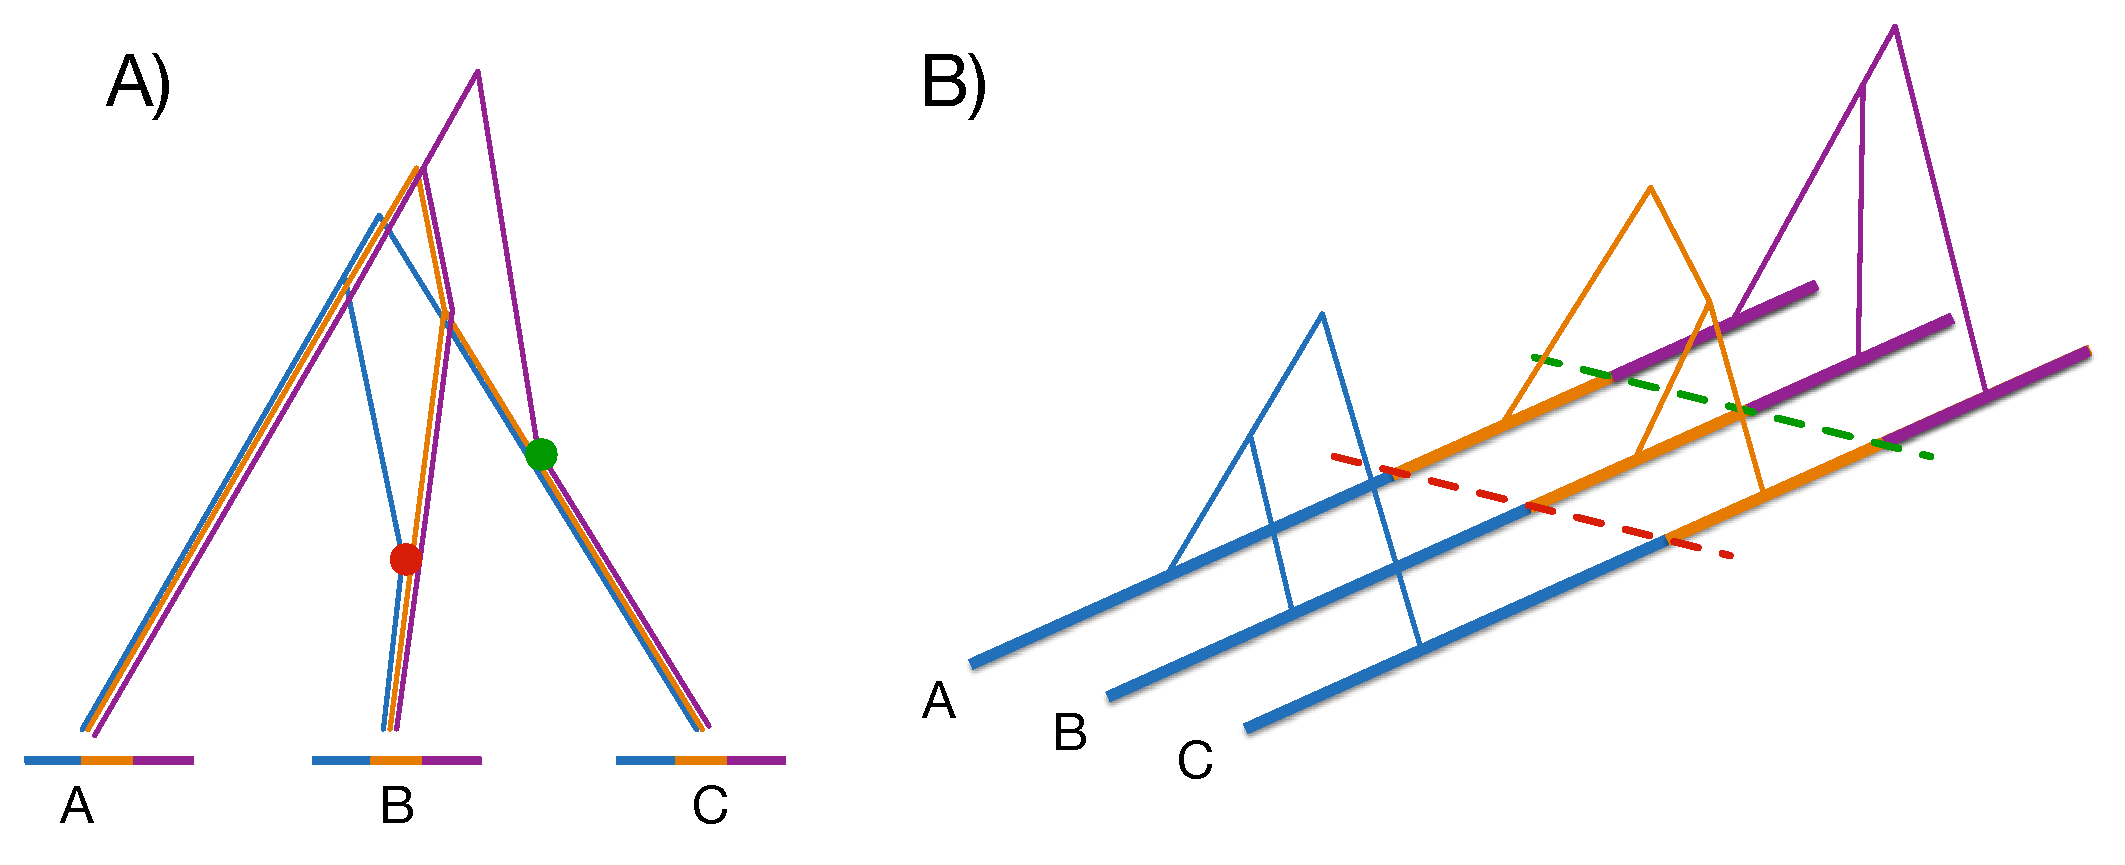
\includegraphics[width=\columnwidth]{Chapters/Sequential-coalescent-figures/ARG-and-local-genealogies}
  \todo[inline]{Use subfigure here instead. Also update it to finite set of nucleotides}
  \caption{A) An ancestral recombination graph over three sequences, showing two recombinations and B) the corresponding three local genealogies. The example shows the ancestry of three sequences in the case where they have experienced two recombination events, shown in red and green. These recombinations segments the sequences into three regions, shown in blue, orange and purple, each with different tree genealogies.}
  \label{fig:ARG-and-local-genealogies}
\end{figure}

There is not a one-to-one correspondence between the local genealogies and the ARG: different ARGs can have exactly the same local genealogies. This is obvious when considering that the timing of recombination events cannot be seen in the local trees. Even ignoring the timing of events there is not a one-to-one correspondence between ARG topologies and the local trees: different ARGs can have the same local trees if recombined lineages coalesce back together in such a way that the local trees do not change. If, for example, a lineage recombines and the two resulting lineages coalesce back again before coalescing with other lineages, this form a ``diamond'' shape in the ARG that is invisible in the local trees. For the purpose of this thesis this is a subtlety we will mostly ignore.

We will be interested in the ARG as a means to generating local trees only and whenever possible either integrate over all ARGs generating the same local trees or even integrate over all ARGs generating the same sequences.


\subsection{Mutations and the likelihood of sampled sequences}

Mutations on lineages can also be considered events in the CTMC, which can occur and modify lineages as the process runs back in time, but typically mutations are put on the coalescence tree or ARG after it is simulated. There, the mutations can simply be put on the genealogy as a Poisson process or be put on inner nodes using a substitution model. The latter approach makes it possible to sum over all possible sequences at internal nodes using standard methods such as Felsenstein's peeling algorithm \cite{Felsenstein_1981} and this way obtain a joint probability distribution for the sequences at the leaves, i.e.\ the present day samples. This distribution depends only on the local tree-genealogies induced by the ARG since the possible nucleotides at any given position only depends on the tree for that given position.

If we denote by $\Theta$ the relevant parameters for the coalescence process, e.g. coalescence rates, migration rates, recombination rates and mutation rates, we can let $f(\G\,|\,\Theta)$ denote the probability density for the process producing the specific genealogy $\G$ and let $f(\A\,|\,\G,\Theta)$ denote the probability that putting mutations on genealogy $\G$ produces the aligned samples $\A$. Typically the alignment probabilities only depends on the mutation rate while the genealogy probabilities is independent of the mutation rate but depends on the coalescence process CTMC and its parameters such as rates (migration, recombination etc.) and time points where it switches between different rate matrices or state spaces.

For demographic inference it is the parameters in $\Theta$ that are of interest rather than the actual underlying genealogy, which is considered a nuisance parameter to be integrated out to get the likelihood
\[
    \lhd(\Theta\,|\,\A) = \int f(\A\,|\,\G) f(\G\,|\,\Theta) \intd\G .
\]

This integral over all possible genealogies is generally not efficiently computable and must either be approximated through sampling approaches or by approximating the coalescence process with a simpler model where the integral \emph{can} be computed. 

In other cases we are interested in inferring the most probable genealogy given the sequence alignment and a fixed set of parameters
\begin{displaymath}
  \argmax_\G f(\G\,|\,\A,\Theta) = 
  \argmax_\G f(\A\,|\,\G) f(\G\,|\,\Theta)
  .
\end{displaymath}

Both of these inference problems can be efficiently solved if we approximate ARG as a sequential Markov process: a coalescence hidden Markov model.

\section{Coalescence hidden Markov models}

The key approximation in coalescence hidden Markov models, or CoalHMMs, is assuming that the distribution of local genealogies along an alignment is Markov. This means that when moving from one tree to another across a recombination point, the next tree depends only on the current tree and not any others. 

By approximating the distribution of local genealogies by a Markov chain the probability of the full genealogy reduces to specifying the joint probability of two neighbouring genealogies (which might be identical genealogies, e.g.\ if there is no recombination between them). Let $\ell$ denote the ``left'' genealogy and $r$ the ``right'' genealogy and $T_\Theta(r \,|\, \ell)$ the ``transition density''. If our data $\A$ consists of $L$ nucleotides then the underlying genealogy $\G=\G_1,\G_2,\ldots,\G_L$  consists of $L$ local trees (where some can be identical) and
\[
    f(\G\,|\,\Theta) = p_\Theta(\G_1) \prod_{i=2}^L T_\Theta(\G_i\,|\,\G_{i-1}) .
\]

The alignment probability given these local genealogies separates into probabilities for the individual nucleotides so if $\A_i$ denotes the $i$'th column in the alignment then
\[
    f(\A\,|\,\G) = \prod_{i=1}^L E_\Theta(\A_i\,|\,\G_i) .
\]
where $E_\Theta(\A_i\,|\,\G_i)$---the ``emission probability''---is the probability that the $\A_i$ column was produced by tree $\G_i$ and can be computed using the peeling algorithm.

In order to integrate over all genealogies we further approximate by discretising the possible time points where inner nodes can be found in the trees. We split the possible coalescence times into $n$ intervals and place all events in the same interval at a single time point. If $p_\Theta(\ell)$ denotes the probability that the left-most tree has the genealogy $\ell$ then we can sum over all possible genealogies
%\begin{equation}
%    \label{eq:integrating-over-genealogies}
%    \begin{split}
%    &\int f(\A\,|\,\G) f(\G\,|\,\Theta) \intd\G =\\
%    &\sum_{\G_1,\ldots,\G_L} \left[ 
%        p_\Theta(\G_1) E(\A_1\,|\,\G_1) 
%        \prod_{i=2}^L T_\Theta(\G_i\,|\,G_{i-1}) E(\A_i\,|\,\G_i)
%    \right] .
%    \end{split}
%\end{equation}
\begin{dmath}
    \label{eq:integrating-over-genealogies}
    \int f(\A\,|\,\G) f(\G\,|\,\Theta) \intd\G = \\
    \sum_{\G_1,\ldots,\G_L} \left[ 
        p_\Theta(\G_1) E(\A_1\,|\,\G_1) 
        \prod_{i=2}^L T_\Theta(\G_i\,|\,G_{i-1}) E(\A_i\,|\,\G_i)
    \right] .
\end{dmath}

This equation takes the form of a hidden Markov model \cite{Rabiner_1989}, where the sequence $\A_1,\ldots,\A_L$ is the observable sequence and $\G_1,\ldots,\G_L$ the hidden Markov sequence.

\subsection{Hidden Markov models}

There is an exponential number of genealogies to sum over in equation \eqref{eq:integrating-over-genealogies}. If there is $N$ possible genealogies local genealogies---genealogies for single loci---and the sequence is $L$ loci long, then the sum is over $N^L$ different sequences of local genealogies. We can rearrange the sum, however, and by applying dynamic programming, the likelihood can be computed in running time $O(N^2L)$.

The algorithm for computing \eqref{eq:integrating-over-genealogies} using dynamic programming is known as the \emph{Forward} algorithm and is part of a suite of algorithms for efficient inference in the framework known as hidden Markov models~\cite{Rabiner_1989,Durbin:2005wq}.

A \emph{hidden Markov model} (HMM) with $N$ ``hidden states'' and $M$ ``observable states'' is defined by a triplet $(T,E,p)$ where $T$ is an $N\times N$ probability matrix (entries are non-negative and rows sum to one), $E$ is an $N\times M$ probability matrix, and $p$ is a $1\times N$ probability vector.

When modelling the ancestry of samples, the hidden states are the local genealogies---that cannot be directly observed---and the observable states are the alignment columns---that \emph{can} be directly observed.

The $p$ vector specifies the probability of starting the hidden sequence in a given state. If $H=(H_1,H_2,\ldots,H_L)$ is a stochastic sequence of hidden states, then $\Pr(H_1=h_1)=p_{h_1}$. The transition matrix, $T$, captures the probabilities for moving through a sequence of hidden states as a Markov process:
\(
    \Pr(H=(h_1,h_2,h_3,\ldots,h_L)) =
    p_{h_1} \cdot \prod_{i=2}^L T_{h_{i-1},h_i}
\). The emission matrix, $E$, specifies the probability of observing state $o_i$ at index $i$ conditional on the hidden state $h_i$ at index $i$: If $O=(O_1,O_2,\ldots,O_L)$ is a stochastic sequence of observable states then 
\(
    \Pr(O=(o_1,\ldots,o_L)\,|\,H=(h_1,\ldots,h_L)) = \prod_i E_{h_i,o_i}
    .
\)

The joint probability of observing both the hidden and the observed sequence is given by
\begin{dmath*}
  \Pr\left(H=(h_1,\ldots,h_L), O=(o_1,\ldots,o_L)\right) =
  p_{h_1} E_{h_1,o_1} \prod_{i=2}^L T_{h_{i-1},h_i} E_{h_i,o_i}
\end{dmath*}
which has the form of the expression inside the sum of equation~\eqref{eq:integrating-over-genealogies}, and not surprisingly the probability of seeing just the observable sequence is
\begin{dmath*}
  \Pr\left(O=(o_1,\ldots,o_L)\right) =
  \sum_{H} \left[
      p_{h_1} E_{h_1,o_1} \prod_{i=2}^L T_{h_{i-1},h_i} E_{h_i,o_i}
  \right]
\end{dmath*}
exactly as equation~\eqref{eq:integrating-over-genealogies}.

The link between the hidden Markov model specification and the coalescence genealogy and alignment probabilities should be obvious: the initial probability vector $p$ is the probability of observing a given genealogy
\begin{dmath*}
    p_i = p_\Theta(\G_i)
\end{dmath*}
the emission matrix is the probability of seeing the alignment column $\A_j$ given the genealogy $G_i$
\begin{dmath*}
    E_{i,j} = E(\A_j\,|\,\G_i)
\end{dmath*}
and the transition probabilities are just
\begin{dmath*}
    T_{i,j} = T_\Theta(\G_j\,|\,\G_i)
    \ .
\end{dmath*}

\subsection{Inference in hidden Markov models}

There is a suite of algorithms for working with hidden Markov models. A thorough treatment of these is beyond the scope of this text but three are worth sketching here: how to compute the likelihood of the parameters given only an observed sequence, how to compute the most probable sequence of hidden states, and how to compute the most probable local genealogy for a given index. These are know as the \emph{Forward} algorithm, the \emph{Viterbi} algorithm, and the \emph{Posterior Decoding}, respectively.

For ease of notation we will use $X_{i:j}$ to mean $(X_i,X_{i+1},\ldots,X_{j})$, i.e.\ the subsequence from $i$ to $j$, for sequences $X$.

\paragraph{The Forward algorithm}

Given a sequence of observable states $o_{1:L}$, the Forward algorithm computes a table of joint probabilities:
\begin{displaymath}
  F[i,h] = \Pr\left(H_i=h, O_{1:i}=o_{1:i}\right)
\end{displaymath}
i.e.\ the table entry $F[i,h]$ contains the probability of observing the prefix of the observed sequence $o_{1:i}$ and being in hidden state $h$ at step $i$. (The probability here is conditional on the three parameters $p$, $T$, and $E$, of the hidden Markov model, but since all probabilities in this section will depend on the same parameters we leave this implicit). This probability is, by the law of total probability, equal to
\begin{equation}
    \label{eq:forward-sum}
  F[i,h] = 
  \sum_{h_{1:i-1}}
  \Pr\left(H_{1:i-1}=h_{1:i-1}, H_i=h, O_{1:i}=o_{1:i}\right)
\end{equation}
which we can rephrase recursively as
\begin{dmath*}[breakdepth=-1]
  F[i,h] 
    =
     \sum_{h_{i-1}}
      \Pr\left(H_i\hiderel{=}h, O_i\hiderel{=}o_i \,|\, H_{i-1}\hiderel{=}h_{i-1}\right)
      \\\quad\times
      \sum_{h_1,\ldots,h_{i-2}}
          \Pr\left(H_{1:i-1}\hiderel{=}h_{1:i-1}, O_{1:i-1}\hiderel{=}o_{1:i-1}\right)
    =
      \sum_{h_{i-1}}
      \Pr\left(H_i\hiderel{=}h, O_i\hiderel{=}o_i 
               \,|\,
               H_{i-1}\hiderel{=}h_{i-1}\right)
             F[i-1,h_{i-1}] 
    =
      \sum_{h_{i-1}} E_{h,o_i} T_{h_{i-1},h} F[i-1,h_{i-1}]
\end{dmath*}
with the special case for $i=1$:
\begin{displaymath}
  F[1,h] = p_h \cdot E_{h,o_1}
  .
\end{displaymath}

Computing the value in each cell takes time $N$---for the sum in the recursion---and there are $N\times L$ cells in the table, so the entire table can be computed in time $O(N^2L)$. Since $F[L,h]$ is the probability of seeing the entire observable sequence and then being in hidden state $h$ we can get the probability of just seeing the observable sequence---applying again the law of total probability---as $\Pr(O)=\sum_h F[L,h]$. This is the likelihood of the observed sequence given the HMM parameters, and the parameters can be estimated by maximising this likelihood.

If we are only interested in the actual sequence likelihood and not the full table, some shortcuts and heuristics can be used to speed up the computations. The algorithm in \citet{Sand:2013bi}, for example---the one we use in likelihood optimisations in the Python framework where we implement our CoalHMMs---exploits that genome alignments consist of very repetitive sequences and preprocess the alignment into a structure where the likelihood can be computed very efficiently.


\paragraph{The Viterbi algorithm}

Instead of computing the probability of the observed sequence, $\Pr(O)=\sum_{H}\Pr(H,O)$, the Viterbi algorithm computes the most probable hidden sequence: $\argmax_H \Pr(H,O)$, (or one such sequence if there are more with the same probability).

The first part of the algorithm follows the Forward algorithm very closely and fills in a table, but for the Viterbi algorithm the table contains the maximum over all possible hidden paths ending in state $h$ rather than the sum over all of them:
\begin{displaymath}
  V[i,h] = 
  \max_{h_{1:i-1}} \Pr\left(H_{1:i-1}=h_{1:i-1}, H_i=h, O_{1:i}=o_{1:i}\right)
\end{displaymath}
and the recursion for computing is identical to the recursion in the Forward algorithm except that maximum is used instead of sum.

Once this table is computed---which like the Forward algorithm can be done in time $O(N^2L)$---we can find the last state in the most likely hidden path as the state $h_L = \argmax_h V[L,h]$ (or one such state if there are ties). From this state we can backtrack the HMM transitions to read off the most likely path.

The most likely second last state is not necessarily the state $h$ that maximises $V[L-1,h]$ since a transition from that state to $h_L$ could potentially be very unlikely. The most likely state at index $L-1$ must be the state $h_{L-1}$ that satisfy $V[L-1,h_{L-1}] T_{h_{L-1},h_L} E_{h_L,o_L} = V[L,h]$ (or an arbitrary such if there are more than one). This state satisfy that, if we have the best possible path that ends in $h_{L-1}$ then taking one more step, to the final state $h_L$, we will have an optimal path (since $h_L$ was selected to be optimal). Scanning through row $L-1$ in $V$ we can thus find the second-last state in the optimal path. We can then repeat this for the third-to-last state and so forth until we have read off the complete optimal hidden path.

In this backtracking phase of the algorithm we need to scan through $N$ states for each of the $L$ positions so the running time is $O(NL)$.


\paragraph{Posterior Decoding}

The Posterior Decoding algorithm calculates the probability of seeing a given hidden state, $h$, at a given position, $i$, conditional on the entire observed sequence: $\Pr(H_i=h\,|\,O=o)$. This can be done for all indices $i$ at the same complexity as computing it for a single index. From this we can read off the most likely hidden state for each position along the sequence, but keep in mind that a sequence of most likely states at each position does not necessarily combine to a most likely complete sequence---or for that matter even a possible sequence.

The posterior probability for seeing state $h$ at position $i$ given the observable sequence $O=o$ can be written as 
\begin{displaymath}
    \Pr(H_i=h\,|\,O=o) = \frac{\Pr(H_i=h,O=o)}{\Pr(O=o)},
\end{displaymath}
where the value $\Pr(O=o)$ is the likelihood we compute with the Forward algorithm, and we have
\begin{dmath*}
    \Pr(H_i=h,O=o) = \\
        \sum_{h_{1:i-1}, h_{i+1:L}} 
        \left.
            \Pr(H_i=h, H_{1:i-1}=h_{1:i-1}, H_{i+1:L}=h_{i+1:L},O=o) 
        \right.
\end{dmath*}
by the law of total probability.

We can further break this up into the sequences before and after position $i$---exploiting along the way that $O_i$ only depends on $H_i$ and not the full hidden sequence---to get
\begin{dmath*}
    \Pr(H_i=h,O=o) = \\
    \sum_{h_{1:i-1}}
    \left.
        \Pr(H_i=h, H_{1:i-1}=h_{1:i-1},O_{1:i}=o_{1:i})
    \right.
    \times 
    \left.
        \sum_{h_{i+1:L}} \Pr(H_{i+1:L}=h_{i+1:L}, O_{i+1:L}=o_{i+1:L}\,|\,H_i=h)
    \right.
\end{dmath*}

The first part of this is the value we compute using the Forward algorithm
\begin{displaymath}
    F[i,h] = \sum_{h_{1:i-1}} \Pr(H_i=h, H_{1:i-1}=h_{1:i-1},O_{1:i}=o_{1:i})
\end{displaymath}
(see eq.~\eqref{eq:forward-sum}), and we can define
\begin{dmath}
\label{eq:backward-sum}
  B[i,h] = 
  \sum_{h_{i+1:L}} 
      \left.\Pr\left(H_{i+1:L}=h_{i+1:L}, O_{i+1:L}=o_{i+1:L}\,|\,H_i=h\right)\right.
  = \left.\Pr\left(O_{i+1:L}=o_{i+1:L}\,|\,H_i=h\right)\right.
\end{dmath}
to get
\begin{displaymath}
  \Pr(H_i=h,O=o) = F[i,h] \cdot B[i,h].
\end{displaymath}

The table $B[i,h]$ defined in eq.~\eqref{eq:backward-sum} can be computed using dynamic programming---very similarly to the table $F[i,h]$---by an algorithm called the Backward algorithm. Both tables $F[i,h]$ and $B[i,h]$ can be computed in time $O(N^2L)$ and after that the posterior distribution at each index can be read off in time $O(N)$.


\subsection{Constructing transition probabilities}

The crux of constructing a CoalHMM---and thereby getting access to the hidden Markov model algorithms for inference---is specifying the probability of transitioning from one local genealogy to another: That is, constructing the transition probability matrix of the hidden Markov model, as a function of the parameters of the coalescence CTMC we aim to approximate. Once this transition matrix is constructed we can obtain the the initial probabilities $p_\Theta$ from marginalisation and the emission probabilities using standard algorithms.

In the literature there are two approaches to computing this transition matrix. Either it is computed by conditioning on the current tree, placing a recombination point on it, and tracking where it can re-coalesce~\cite{Hobolth:2014cw,Li:2011ez} or it is computed by considering the joint distribution of two neighbouring trees~\cite{Dutheil:2009dt,Mailund:2011dv}. The latter is the approach we will consider in this thesis.

Let $J_\Theta(\ell,r)$ denote the joint probability of seeing the genealogy $\ell$ on the left and $r$ on the right of two nucleotides. Then the transition probability is given by
\[
    T_\Theta(r \,|\, \ell) = \frac{J_\Theta(\ell,r)}{p_\Theta(\ell)}
\]
and the initial probabilities given by
\[
    p_\Theta(\ell) = \sum_{r} J_\Theta(\ell, r)
    .
\]

The probabilities $J_\Theta(\ell,r)$ can be computed using continuous time Markov chains tracking the ancestry of two neighbouring nucleotides, which is the topic of the following chapters.

\chapter{Modelling the ancestry of two neighbouring nucleotides}
\label{chap:modelling-2-ARGs}

To build the hidden Markov model transition probabilities we need to construct the joint probability matrix, $J_\Theta(\ell,r)$, of two neighbouring genealogies $\ell$ and $r$. The approach we take is to construct these probabilities using continuous time Markov chains (CTMCs). By specifying how samples of sequences of length two trace their ancestry back in time in a CTMC we can get a probability distribution of all possible genealogies. This chapter covers how we can construct these CTMCs. Chapters~\ref{chap:composing-CTMCs}~and~\ref{chap:constructing-coalhmms} will cover how we translate the CTMCs into CoalHMMs.

\section{A transition system for tracing ancestry}

The approach we take explicitly enumerates all possible ancestral states the sampled lineages can reach back in time and all possible transitions between them. Constructing this state space by hand is both tedious and error prone. The number of states and transitions grows super-exponential in the number of samples handled or the number of populations modelled, so automatic generation of the state space is essential.

To automatically generate the state space for a demographic model we need to specify a small set of rules for how the state space should be constructed and then implement an algorithm for constructing the full set of states and transitions these rules are describing. There are many formal ways of describing such rules for generating a state space. Here we will, inspired by \citet{springerlink:10.1007/978-3-642-31131-4_3}, consider a system based on \emph{coloured Petri nets}.

\subsection{Coloured Petri nets}

Petri nets is a formalism for describing the evolution of a concurrent system in terms of a so-called token game. A Petri net consist of a set of ``places'' where tokens can be placed, and a state of the system is defined by the number of tokens on each place. The system then evolves by the occurrence of ``transitions'', where each transition removes a fixed number of tokens from some of the places and places other tokens on other places.

Coloured Petri nets extend Petri nets by assigning information (colours) to the tokens. Tokens are still placed on places and transitions still remove existing tokens and put down new tokens; now, however, there is data associated with each token. Below I will give a simplified definition of coloured Petri nets, sufficient for the needs of the system we need to build for the coalescence process. For a more comprehensive treatment of coloured Petri nets I refer to \citeauthor{Jensen:2009ti} ``\citetitle{Jensen:2009ti}''~\cite{Jensen:2009ti}. Readers already familiar with coloured Petri nets might want to skip to the next section as I am taking some liberties in how I formalise nets; this is done to avoid complications that are irrelevant for our needs here.\footnote{The definition I give of coloured Petri nets is much simplified compared to the defintion in \citet{Jensen:2009ti}. I do not bother with formally defining the types associated with places, just assign a set to each place, nor distinguish between transitions and transition bindings but lump them together so what I call transitions here really corresponds to bindings in \citet{Jensen:2009ti}. Since we will not need to have more than one token of any color on the same place I do not use multi-sets but simply sets.}

Formally we define a coloured Petri net as a tuple $(P,T,C,\pre,\post)$ where $P$ is a set of \emph{places} and $T$ is a set of \emph{transitions}. $C$ is a $P$ indexed set of set and we say that $C(p)$ is the (colour) type of place $p\in P$. A \emph{marking} or state of a coloured Petri net is defined by which \emph{tokens} are found on each place. Formally it is a mapping $m$ that maps each place $p$ to a set $m(p)\subseteq C(p)$. Elements in $m(p)$ are the tokens placed on place $p$ in the given marking or state.

Finally, $\pre$ and $\post$ are mappings that determines how the system can evolve. For each transition, $\pre$ specifies which tokens the transition will consume---and therefore which tokens must be present on in the current marking for the transition to be possible---and $\post$ specifies which tokens the transition will produce. For all transitions $t$ and places $p$, $\pre(t,p) \subseteq C(p)$. A transition $t$ is possible, or \emph{enabled}, in a marking $m$ if for all places $p$ $\pre(t,p)\subseteq m(p)$, i.e.\ if all the tokens that the transition will consume at any place are on the place in the marking. For all transitions $t$ and places $p$, $\post(t,p) \subseteq C(p)$ determines which tokens are produced by the occurrence of transition $t$. If $m$ is the current marking and transition $t$ is enabled, then the occurrence of transition $t$ will update the marking to $m'$ satisfying $\forall p: m'(p) = m(p) \setminus \pre(t,p) \cup \post(t,p)$, i.e.\ we remove the tokens in $\pre(t,p)$ and then add the tokens in $\post(t,p)$. If transition $t$ is enabled in marking $m$ and its occurrence would lead to marking $m'$ we write this as $m[t\rangle m'$. We will write $m[t_1,t_2,\ldots,t_k\rangle m'$ if there exists intermediate states $m_i,i=1,\ldots,k$ such that $m_{i-1}[t_i\rangle m_i$ with $m_0=m$ and $m_k=m'$ and $m[\cdots\rangle m'$ if there exists a sequence of transitions $t_1,\ldots,t_k$ such that $m[t_1,\ldots,t_k\rangle m'$. We will also allow this sequence of transitions to be empty so $m[\cdots\rangle m$.

\subsection{A coloured Petri net of the coalescence process}

To construct our coalescence system as a coloured Petri net, we let $\samples=\{s_1,s_2,\ldots,s_n\}$ denote a set of samples for the system and let $\populations=\{p_1,p_2,\ldots,p_m\}$ denote a set of populations. We do not necessarily require that there is a sample from each population or that all samples will be able to migrate to all populations, but because of the state space explosion problem we should not model more populations than strictly necessary.

The Petri net we construct will only need a single place. We want tokens to represent ancestral lineages, so we want them to hold information about which population a given lineage is in, and which present day samples they are ancestral to, on both the left and the right nucleotide. The colour set of the place will therefore be $\populations\times\powerset(\samples)\times\powerset(\samples)$, where $\powerset(\samples)$ denotes the power set of samples, i.e.\ the set of all subsets of $\samples$. The first component specifies the population, of which there can be only one, and the next two the set of samples the lineage is ancestral to on the left and on the right, respectively. Since we only have a single place, we will not include it in the notation for the $\pre$ and $\post$ sets and write $\pre(t)$ and $\post(t)$ instead of $\pre(t,p)$ and $\post(t,p)$.

We will have three kinds of transitions: \emph{coalescence}, \emph{migration}, and \emph{recombination} transitions. Figure~\ref{fig:ctmc-cpn} is a graphical representation of these transitions. Here, the rectangular nodes represent the three types of transitions, the oval node the single place, and the arcs between them represent the $\pre$ and $\post$ mappings. Arcs from the place to a transition represent the $\pre$ mapping and arcs from a transition to a place the $\post$ mapping. The inscriptions on the arcs describe the lineages/tokens that a transition will consume and produce. There are concrete transitions for each assignment of values to the variables on these arc inscriptions.

Coalescence transitions are indexed by the values for two tokens, $(p_i,\ell_i,r_i),(p_j,\ell_j,r_j)\in\populations\times\powerset(\samples)\times\powerset(\samples)$, but will require that the tokens are in the same population, $p_i = p_j$. For each assignment of values to these variables we have a coalesce transition $\coaltrans(p_i,\ell_i,r_i,\ell_j,r_j)$. The $\pre$ set, the set of tokens to be consumed, is
\[
    \pre(\coaltrans(p_i,\ell_i,r_i,\ell_j,r_j)) =
    \{\,(p_i,\ell_i,r_i),\,(p_i,\ell_j,r_j)\,\}
    ,
\]
and a coalescence transition will merge the left and right ancestral lineages so the new token it produces is
\[
    \post(\coaltrans(p_i,\ell_i,r_i,\ell_j,r_j)) =
    \{\,(p_i,\,\ell_i\cup\ell_j,\,r_i\cup r_j)\,\}
    .
\]

There is no difference between the first and the second token selected here, so we consider $\coaltrans(p_i,\ell_i,r_i,\ell_j,r_j)$ and $\coaltrans(p_j,\ell_j,r_j,\ell_i,r_i)$ the same transition.

\begin{figure}[tb]
  \missingfigure{The CPN for the coalescence system}
  \caption{A coloured Petri net for the coalescence system.
  The oval node represents the single place of the Petri net and the rectangular nodes the different transitions. Each type of transition is only shown as a single node but the annotations on the arcs between transitions and the place, representing the $\pre$ and $\post$ mappings, can take different values representing different instances of the transitions.}
  \label{fig:ctmc-cpn}
\end{figure}

Migration transitions are indexed by two populations, $p_i \neq p_j$ and a token from one of them $(p_i,\ell_i,r_i)$. It will consume the token in population $p_i$ and produce a new token in population $p_j$ with the same ancestral lineages:
\[
    \pre(\migtrans(p_i,p_j,\ell_i,r_i) =
    \{\,(p_i,\ell_i,r_i)\,\}
    ,
\]and\[
    \post(\migtrans(p_i,p_j,\ell_i,r_i) =
    \{\,(p_j,\ell_i,r_i)\,\}
    .
\]

If we only want to permit migration between certain pairs of populations, or if we want migration in only one direction, we can restrict further the possible migration transitions accordingly.

Recombination transitions are indexed by a single token that they consume and instead produce two tokens, one containing the ancestral lineages on the left of the consumed transition and one containing the ancestral lineages on the right:
\[
    \pre(\recombtrans(p_i,\ell_i,r_i) =
    \{\,(p_i,\ell_i,r_i)\,\},
\]
and
\[
    \post(\recombtrans(p_i,\ell_i,r_i) =
    \{\,(p_i,\ell_i,\emptyset),\,(p_i,\emptyset,r_i)\,\}
    .
\]

When considering markings for this net we will just refer to the set associated with the single place; instead of describing a mapping from places to their colour set, we simply refer to the tokens on that place.

\subsection{Example}

As an example, consider a case with two populations $\populations=\{\,p_1,\,p_2\,\}$ and two samples $\samples=\{\,s_1,\,s_2\,\}$. We imagine we obtained these samples such that sample $s_1$ came from population $p_1$ and sample $s_2$ from population $p_2$, so with an initial marking 
\[
    m_\iota = \{\,(p_1,\{s_1\},\{s_1\}),\,(p_2,\{s_2\},\{s_2\})\,\}
    .
\]

Four transitions are possible in this initial state. Either of the two lineages can recombine:
\begin{eqnarray}
    \label{eq:recomb_transition_1}
    m_\iota
    \quad \big[\recombtrans(p_1,\{s_1\},\{s_1\})\big\rangle \quad
    \{\,(p_1,\{s_1\},\emptyset),\,
        (p_1,\emptyset,\{s_1\}),\,
        (p_2,\{s_2\},\{s_2\})\,\}\\
    \label{eq:recomb_transition_2}
    m_\iota
    \quad \big[\recombtrans(p_2,\{s_2\},\{s_2\})\big\rangle \quad
    \{\,(p_1,\{s_1\},\{s_1\}),\,
        (p_2,\{s_2\},\emptyset),\,
        (p_2,\emptyset,\{s_2\})\,\}
\end{eqnarray}
and either lineage can migrate to the other population
\begin{eqnarray}
    \label{eq:migration_transition_12}
    m_\iota
    \quad \big[\migtrans(p_1,p_2,\{s_1\},\{s_1\})\big\rangle \quad
    \{\,(p_2,\{s_1\},\{s_1\}),\,(p_2,\{s_2\},\{s_2\})\,\}\\
    \label{eq:migration_transition_21}
    m_\iota
    \quad \big[\migtrans(p_2,p_1,\{s_2\},\{s_2\})\big\rangle \quad
    \{\,(p_1,\{s_1\},\{s_1\}),\,(p_1,\{s_2\},\{s_2\})\,\}
\end{eqnarray}

There are no coalescence transitions possible in the initial state since the two lineages are in separate populations. If, however, the transition in \eqref{eq:recomb_transition_1} occurred there would be two lineages, $(p_1,\{s_1\},\emptyset)$ and $(p_1,\emptyset,\{s_1\})$ in population $p_1$ that could coalesce back into the initial marking
\[
    \{\,(p_1,\{s_1\},\emptyset),\,
        (p_1,\emptyset,\{s_1\}),\,
        (p_2,\{s_2\},\{s_2\})\,\}
    \quad
    \big[\coaltrans(p_1,\{s_1\},\emptyset,\emptyset,\{s_1\})\big\rangle 
    \quad
    m_\iota
    .
\]

Similarly, if the transition in \eqref{eq:recomb_transition_2} occurred, a coalescence transition for the two lineages in population $p_2$ would be enabled for taking the system back to its initial state.

Transitions \eqref{eq:migration_transition_12} and \eqref{eq:migration_transition_21} both move a lineage from one population to another; after either of these transitions a coalescence transition is also enabled. If the transition in \eqref{eq:migration_transition_12} occurred, both lineages are in population $p_2$ and the coalescence transition $\coaltrans(p_2,\{s_1\},\{s_1\},\{s_2\},\{s_2\})$ is enabled. If this transition then occurs it will update the marking to
\(
    \{\,(p_2,\,\{s_1,s_2\},\,\{s_1,s_2\})\,\}
    ,
\)
which contains a single lineage that holds the ancestral material for both samples.

A possible run of this process, from the initial state until all lineages have found their most recent common ancestor, could look like this:
\begin{align}
    \nonumber
    m_\iota &= \{\,(p_1,\{s_1\},\{s_1\}),\,(p_2,\{s_2\},\{s_2\})\,\}
    \\ %% recombination
    &\big[\recombtrans(p_1,\{s_1\},\{s_1\})\big\rangle
    \label{eq:ex_recomb_1}
    \\
    \nonumber
    &
    \{\,(p_1,\{s_1\},\emptyset),\,
        (p_1,\emptyset,\{s_1\}),\,
        (p_2,\{s_2\},\{s_2\})\,
    \}
    \\ %% migration
    &\big[\migtrans(p_1,p_2,\{s_1\},\emptyset)\big\rangle
    \label{eq:ex_mig_1}
    \\
    \nonumber
    &
    \{\,(p_2,\{s_1\},\emptyset),\,
        (p_1,\emptyset,\{s_1\}),\,
        (p_2,\{s_2\},\{s_2\})\,
    \}
    \\ %% coalescence
    &\big[\coaltrans(p_2,\{s_1\},\emptyset,\{s_2\},\{s_2\})\big\rangle
    \label{eq:ex_coal_1}
    \\
    \nonumber
    &
    \{\,(p_1,\emptyset,\{s_1\}),\,
        (p_2,\{s_1,s_2\},\{s_2\})\,
    \}
    \\ %% migration
    &\big[\migtrans(p_2,p_1,\{s_1,s_2\},\{s_2\})\big\rangle
    \label{eq:ex_mig_2}
    \\
    \nonumber
    &
    \{\,(p_1,\emptyset,\{s_1\}),\,
        (p_1,\{s_1,s_2\},\{s_2\})\,
    \}
    \\ %% coalescence
    &\big[\coaltrans(p_1,\emptyset,\{s_1\},\{s_1,s_2\},\{s_2\})\big\rangle
    \label{eq:ex_coal_2}
    \\
    \nonumber
    &
    \{\,
        (p_1,\{s_1,s_2\},\{s_1,s_2\})\,
    \}
\end{align}

First, the lineage in population $p_1$ recombines into two lineages, \eqref{eq:ex_recomb_1}, after which the lineage carrying the left nucleotide for sample $s_1$ migrations into population $p_2$, \eqref{eq:ex_mig_1}. The two lineages now in population $p_2$ coalesces, \eqref{eq:ex_coal_1}, before migrating to population $p_1$, \eqref{eq:ex_mig_2}, and finally coalescing with the right nucleotide of sample $s_1$, \eqref{eq:ex_coal_2}.

\begin{figure}[tb]
  \missingfigure{Example ancestral recombination graph}
  \caption{Example ancestral recombination graph. The graph shows the ancestral lineages and events of transitions, described in the main text, going back in time from the present until the most recent common ancestor for both left and right nucleotides of the two lineages.}
  \label{fig:cpn-arg}
\end{figure}


\section{From the reachability graph to a CTMC}

Given an \emph{initial marking} $m_\iota$ the state space of a coloured Petri net consists of all states reachable from this state (markings $m$ where $m_\iota[\cdots\rangle m$) and all possible transitions between reachable states (i.e.\ between markings $m$ and $m'$ we have all transitions $t$ with $m[t\rangle m'$). It is from this state space we construct the continuous time Markov chain that will give us the probability density over all pairs of genealogies.

To specify the CTMC for the ancestry of our samples we need only specify the rate matrix $Q$ and the initial state probabilities $\pi(0)$. The latter is the simplest; if $\iota$ denotes the index of the initial marking then $\pi(0)_i = 1$ if $i=\iota$ and $\pi(0)_i = 0$ if $i\neq\iota$. The former, specifying the rate matrix $Q$, requires a traversal of all the transitions in the state space. Once we know how many states there are, say $N$, then we can allocate a matrix of size $N\times N$ and initially set all entries to zero. We then need to enumerate all states $m$ and assign them an index $i_m$. For all transitions $m[t\rangle m'$ we then need to assign to $Q_{i_m,i_{m'}}$ the rate for transition $t$. These rates, e.g.\ the coalescence rate in population $p$ or the migration rate between populations $p$ and $q$, are parameters of the model and must be looked up in a table. Once all the off-diagonal entries are filled in, the diagonal is assigned minus the row sums.

\section{Implementing the state space generator}


It is relatively straightforward to implement the state space generator for the coloured Petri net described above. All transitions are relatively simple, consuming either one or two tokens, and all tokens\todo{check if I have introduced tokens in the text above} are of a very simple type. In the IMCoalHMM framework the state space generator is implemented in a class with two key methods. The first is responsible for computing the successors for any given state and the second for generating the complete reachability graph and then the CTMC rate matrix for the system.

The computation of successor states is done as shown below:

\begin{lstlisting}
    def successors(self, state):
        tokens = list(state)

        # Transitions consuming one token.
        for ttype, tfunc in self.transitions[0]:
            for token in tokens:
                pre = frozenset([token])
                for pop_a, pop_b, post in tfunc(token):
                    pop_a, pop_b, post = result
                    new_state = state.difference(pre).union(post)
                    yield ttype, pop_a, pop_b, new_state

        # Transitions consuming two tokens.
        for ttype, tfunc in self.transitions[1]:
            for i in xrange(len(tokens)):
                for j in xrange(i):
                    pre = frozenset([tokens[i], tokens[j]])
                    for pop_a, pop_b, post in tfunc(tokens[i], tokens[j]):
                        new_state = state.difference(pre).union(post)
                        yield ttype, pop_a, pop_b, new_state
\end{lstlisting}

The method takes the lineages in the state --- here called ``tokens'' in the terminology of Petri nets --- and considers each single token in turn for each possible transition that consumes a single token (these are kept in the list \texttt{self.transitions[0]}) --- or all possible pairs of tokens for each possible transition that consumes two tokens (these are kept in the list \texttt{self.transitions[1]}). In the description of the Petri net above there are three types of transitions --- recombination and migration that consumes one token and coalescence that consumes two --- but the code is more general and can easily be extended to have more transitions.

The protocol for transitions is that they consist of a type (\texttt{ttype}) --- used to identify them when we need to annotate edges in the reachability graph and assign rates to entries in the rate matrix --- and a function (\texttt{tfunc}) responsible for computing the possible products of the transition. The function actually returns a list of possible products. This is used both to handle cases where more than one output is possible --- for migration transitions the same lineage can migrate to more than one population so more than one possible product is possible --- or to abort a transition (return an empty list) to avoid transitions we do not want to allow --- such as recombinations where either the left or right nucleotide is the empty set.

 The transition function returns two populations as well; the purpose is to identify the transition if rates depend on the populations of the tokens involved. For the transitions we have considered, only migration transitions actually involve two populations, but rather than handling two cases --- one or two populations associated with a transition --- the protocol is just to let all transitions return two populations.

It is possible for the transition function to return \texttt{None} as a way of aborting the transition. This is used by recombination transitions to avoid recombinations on lineages where either the left or right nucleotides are the empty set.

For each transition, a successor state is computed by removing the token(s) in the pre-set of the transition and adding the post-set of tokens.

The transitions are listed below. The first two consume a single token and are stored in \texttt{self.transitions[0]} and the third consumes two tokens and is stored in \texttt{self.transitions[1]}.

The recombination transition first checks that both left and right nucleotide contains ancestral material. If they do not it returns the empty list, and no successor states will be computed for that transition. If they do, it returns two tokens, one with the left ancestral material and one with the right ancestral material. Only a single population is involved, so it just returns that population twice.

\begin{lstlisting}
    def recombination(token):
        pop, left, right = token
        if not (left and right): return [] # Abort transition
        return [(pop, pop, frozenset([(pop, left, frozenset()),
                                      (pop, frozenset(), right)]))]
\end{lstlisting}

The migration transition consumes a single token and produce a list of tokens for all other populations than the one the token was originally in. (The listing here is slightly simplified compared to the implementation in the framework --- there the state space generator has a table of populations that it allows migrations between so we do not have to allow all possible migrations --- but the implementation below is closer to the description above).

\begin{lstlisting}
    def migrate(self, token):
        pop, left, right = token
        res = [(pop, pop2, frozenset([(pop2, left, right)]))
               for pop2 in self.populations if pop2 != pop]
        return res	
\end{lstlisting}

Finally, the coalescence transition takes two tokens. If they are from different populations it aborts and if not it constructs a new token by joining the two left and the two right sets.

\begin{lstlisting}
    def coalesce(token1, token2):
        pop1, left1, right1 = token1
        pop2, left2, right2 = token2
        if pop1 != pop2: return [] # Abort transition
        left, right = left1.union(left2), right1.union(right2)
        return [pop1, pop2, frozenset([(pop1, left, right)])]
\end{lstlisting}

\newpage % FIXME: FOR LAYOUT -- CHECK HOW IT LOOKS IF YOU CHANGE THE TEXT
The computation of the state space is then handled by the method listed below:
\begin{lstlisting}
    def compute_state_space(self):

        if type(self.init) == list:
            seen = set(self.init)
            unprocessed = list(self.init)
            self.state_numbers = dict((x,i) for i, x in enumerate(self.init))
        else:
            seen = {self.init}
            unprocessed = [self.init]
            self.state_numbers = {self.init: 0}

        edges = []

        # Construct the reachability graph
        while unprocessed:
            state = unprocessed.pop()
            state_no = self.state_numbers[state]
            for trans, pop1, pop2, dest in self.successors(state):
                if dest not in self.state_numbers:
                    self.state_numbers[dest] = len(self.state_numbers)
                if dest not in seen:
                    unprocessed.append(dest)
                    seen.add(dest)
                edges.append((state_no,
                              (trans, pop1, pop2),
                              self.state_numbers[dest]))

        # Collect transitions so they map between state indices
        remapping = {}
        mapped_state_numbers = {}
        for state_no in set(self.state_numbers.values()):
            remapping[state_no] = len(remapping)
        for state, state_no in self.state_numbers.iteritems():
            mapped_state_numbers[state] = remapping[state_no]

        self.states = mapped_state_numbers
        self.transitions = [(remapping[src], (trans, pop1, pop2), remapping[dest])
                            for src, (trans, pop1, pop2), dest in edges]

\end{lstlisting}

It first handles a special case for initial states. In the description above we have considered a single initial state for a system, and in general that will also be the case. All the coalescence systems we consider have a single initial state at time zero. However, sometimes we have to handle systems where it is possible to start in different states --- this happens when we have different systems further back in the past where the evolution back to that time can leave the system in different states. The need for this should become clearer in later chapters; for now it is perhaps best just to consider it a technical detail.

Once the initial state(s) is handled, the reachability graph construction is straightforward: each state is considered in turn and all its successor are computed. We collect the transitions from the state to all its successors and those successors we have not seen before we add to a list of unprocessed states to be handled later (and record that we have now seen them).

When building the reachability graph we need to represent states as sets of tokens, but once we are done we want to represent them simply as indices in the CTMC rate matrix we will need to build, so after building the graph we map all states to their numbers and collect the transitions in a form that goes from index to index rather than from state to state.

From the reachability graph we can now very easily build the CTMC rate matrix. Given a table of rates, \texttt{rates_table}, where we can look up the numerical value for the rate of a transition --- where a transition is represented by the transition type and the two populations involved --- the computation can be done as this:

\begin{lstlisting}
  rate_matrix = matrix(zeros((len(state_space.states),
                              len(state_space.states))))

  for src, trans, dst in state_space.transitions:
      rate_matrix[src, dst] = rates_table[trans]

  for i in xrange(len(state_space.states)):
      rate_matrix[i, i] = - rate_matrix[i, :].sum()
\end{lstlisting}

We do not do this in the state space module, however. For each choice of model parameters the rates can change so we will need to recompute the rate matrix several times in model fitting. The reachability graph, however, is fixed for the system so we compute this only once and store it in the symbolic form above and then build the CTMC rate matrix when we need it in the likelihood computations.

The rates table depends on the actual demographic model. For a two population model it could be constructed by a function as that below:
\begin{lstlisting}
def make_rates_table_migration(coal_rate_1, coal_rate_2, recomb_rate,
                               migration_rate_12, migration_rate_21):
    table = dict()
    table[('C', 1, 1)] = coal_rate_1
    table[('C', 2, 2)] = coal_rate_2
    table[('R', 1, 1)] = recomb_rate
    table[('R', 2, 2)] = recomb_rate
    table[('M', 1, 2)] = migration_rate_12
    table[('M', 2, 1)] = migration_rate_21
    return table
\end{lstlisting}
where 'C', 'R', and 'M' are used as the function types and 1 and 2 to identify the populations.


\section{The state space explosion problem}

\todo[inline]{Statistics on how the state space explodes}


\chapter{Joining CTMCs spanning different time periods}
\label{chap:composing-CTMCs}

The continuous time Markov chains we use to model a coalescence system captures a fixed number of populations with fixed rates of coalescence within them and migration between them. To construct more complex demographic scenarios---e.g.\ merging and splitting of populations or entering and leaving migration periods---we combine such CTMCs so different models are used for different time periods.

If one CTMC, $\{\,X(t)\;|\;\tau>t\geq 0\,\}$, models the system before time $\tau$ and another, $\{\,Y(t)\;|\;t\geq\tau\,\}$, models the system after time $\tau$, we need a way of relating the states between the two CTMCs. If $\pi(t)$ is the state probability vector then it potentially assign probabilities to two different sets of states before and after time $\tau$, and we need a way of relating the vector $\pi(\tau-\epsilon)$ to the vector $\pi(\tau+\epsilon)$.

A natural way to map vectors from one state space to another is using a matrix. If $\pi_X(t)$ is the probability vector for CTMC $X$ with $N_X$ states, and $\pi_Y(t)$ the probability vector for CTMC $Y$ with $N_Y$ states, we use $\pi_X(t)$ for the time interval $[0,\tau)$ and $\pi_Y(t)$ for the time interval $[\tau,\infty)$. We map between them by setting $\pi_Y(\tau)=\pi_X(\tau)\cdot\eta$ where $\eta$ is an $N_X\times N_Y$ matrix with non-negative values and where each row sums to $1$ so probabilities are preserved.

The mapping matrix $\eta$ is part of the demographic model and to specify such mappings between two consecutive time periods we develop a small meta-language.

\section{Mapping lineages and states}

Recall from chapter~\ref{chap:modelling-2-ARGs} that the state of the coalescent system CTMC consist of a set of lineages $(p,\ell,r)$ where $p$ is a population and $\ell$ and $r$ are sets of samples. The simplest case for mapping states maps lineages individually. The mapping between states is then derived from the mapping between lineages simply by applying the lineage map over all lineages in the state. If we let
\begin{displaymath}
  \lambda: \populations\times\powerset(\samples)\times\powerset(\samples)
      \to \populations\times\powerset(\samples)\times\powerset(\samples)
\end{displaymath}
denote the mapping between lineages we can define a mapping between states
\begin{displaymath}
  \sigma_\lambda: 
  \powerset\Big(\populations\times\powerset(\samples)\times\powerset(\samples)\Big)
      \to 
  \powerset\Big(\populations\times\powerset(\samples)\times\powerset(\samples)\Big)
\end{displaymath}
between states by $\sigma_\lambda(x) = \big\{\,\lambda(l)\;\big|\;l\in x\,\big\}$.

When the state mapping is defined this way---where one lineage is mapped to one lineage---each state in the first CTMC is mapped to exactly one state in the next CTMC. Each row in $\eta$ will therefore contain a single cell containing $1$ and all other cells will be $0$.


\paragraph{An isolation model}

To illustrate the mapping between CTMCs we consider the simple isolation model shown in figure~\ref{fig:demographic-model-isolation-model} and developed in \citet{Mailund:2011dv}. The model has two different time periods. From the present and back until time $\tau$ it consists of two isolated populations, $p_1$ and $p_2$, and further back in time it consists of a single ancestral population, $p_A$.

\begin{figure}[tb]
  \missingfigure{Illustration of isolation model}
  \caption{A two-population isolation model. Two populations are completely isolated from the present and back to time $\tau$ in the past where they separated from an ancestral population.}
  \label{fig:demographic-model-isolation-model}
\end{figure}

We naturally model this as two CTMCs. We have the isolation system $\{\,I(t)\;|\;\tau > t \geq 0\,\}$ and the ancestral system $\{\,A(t)\;|\;t\geq\tau\,\}$. We assume that we have one sample from each population, initially with the left and right nucleotides sitting on the same chromosome. In the isolation system the lineages can recombine and coalesce within the separate populations. At time $\tau$ the two populations merge (when looking back in time) and lineages from population $p_1$ and $p_2$ now must become lineages in the ancestral population, $p_A$, where they can recombine and coalesce and find common ancestors.

Moving from the isolation system to the ancestral population we must map the lineages in the two separated populations into the ancestral population. In this model each state in the isolation system corresponds uniquely to one state in the ancestral system. The lineages are preserved; only the populations change. The lineage map is thus defined as $\lambda: (p_i,\ell,r) \mapsto (p_A,\ell,r)$ for $i=1,2$.


\paragraph{An isolation-with-initial-migration model}

As a second example consider the isolation-with-initial migration model in figure~\ref{fig:demographic-model-IIM-model}, developed in \cite{Mailund:2012ew}. This model is very similar to the isolation model but has three different time periods. An isolation period and an ancestral population as has the isolation model, and in between a period where lineages can migrate between the two populations.

\begin{figure}[tb]
  \missingfigure{Illustration of IIM model}
  \caption{A two-population isolation-with-initial-migration model. Two populations are completely isolated from the present and back to time $\tau_1$ in the past. From $\tau_1$ to $\tau_2$ migration between the two populations is possible, and at $\tau_2$ the two populations merge into an ancestral population.}
  \label{fig:demographic-model-IIM-model}
\end{figure}

Mapping from the isolation to the migration period and from migration to the ancestral population period in this model can also be done using just a lineage map.

The state space for the isolation period is a subset of the state space of the migration period; it consists of the states where lineages originating in population $p_1$ remains in population $p_1$ and lineages originating in population $p_2$ remains in population $p_2$. The migration state space contains these states as well as those where lineages from $p_1$ are now in $p_2$ and those from $p_2$ are now in $p_1$. When entering the migration period from the isolation period, however, the lineages in population $p_1$ will still be in population $p_1$---they will need to migration before that changes---and lineages in population $p_2$ will still be in population $p_2$. The lineage map is therefore just the identity function: $\lambda: (p_i,\ell,r)\mapsto(p_i,\ell,r)$ for $i=1,2$.

Going from the migration period to the ancestral population we need to map all lineages from the two separate populations into the ancestral, exactly as we did for the isolation model: $\lambda: (p_i,\ell,r)\mapsto (p_A,\ell,r)$ for $i=1,2$. The only difference from the isolation model is that the lineages that originated in one population can now be in another, so the corresponding state map, $\sigma_\lambda$, maps from a larger state space than in the case of the isolation model. Since we only have to worry about how individual lineages are mapped, the specification does not get more complicated by this.

\paragraph{} % This is here to make some space between this and the example
We cannot always construct the mapping matrix by a one-to-one translation of lineages. Even so, we are often far from the completely general case, where the mapping matrix $\eta$ can be completely arbitrary (within the restrictions preserving probabilities), since most modelling still considers lineages individually. Typically, a single lineage before the change in state space maps to different lineages after the change---with different probabilities---but still where each lineage is placed after the change is independent of all other lineages before the change.

Consider a state with a single lineage $(p,\ell,r)$ in the system before the change. If this lineage can map to a number of different lineages, $(p_1,\ell_1,r_1)$, $(p_2,\ell_2,r_2)$, $\ldots$, $(p_k,\ell_k,r_k)$ in the system after the change, with probabilities $\alpha_1,\ldots,\alpha_k$, we want the system mapping $\eta$ to map the single lineage state to $k$ different states such that we transition into the state with lineage $(p_i,\ell_i,r_i)$ with probability $\alpha_i$.

Consider now a state with two lineages, $(p,\ell,r)$ and $(q,s,t)$, where the first lineage maps into lineages $(p_1,\ell_1,r_1)$, $\ldots$, $(p_k,\ell_k,r_k)$ with probabilities $\alpha_1, \ldots, \alpha_k$ and $(q,s,t)$ maps into lineages $(q_1,s_1,t_1)$, $\ldots$, $(q_m,s_m,t_m)$ with probabilities $\beta_1,\ldots,\beta_m$. If the mapping of individual lineages are independent, then $\eta$ should map this state into a state with lineages $(p_i,\ell_i,r_i)$ and $(q_j,s_j,t_j)$ with probability $\alpha_i\cdot\beta_j$.

In general we can consider a state, $S=\{(p_i,\ell_i,r_i)\,|\,i=1,\ldots,n\}$, and say that  each lineage $(p_i,\ell_i,r_i)\in S$ maps to a set of lineages $\lambda(p_i,\ell_i,r_i)=\{(p_{i,1},\ell_{i,1},r_{i,1}),\ldots,(p_{i,k},\ell_{i,k},r_{i,k})\}$ and a set of probabilities $\{\alpha_{i,1},\ldots,\alpha_{i,k}\}$ indexed such that $\alpha_{i,j}$ is the probability that lineage $(p_i,\ell_i,r_i)$ maps to $(p_{i,j},\ell_{i,j},r_{i,j})$. If we consider all the lineages in $S$, the states that $S$ can map to are all the states where each lineage $(p_i,\ell_i,r_i)$ is mapped to exactly one lineage in $\lambda(p_i,\ell_i,r_i)$.

For any such selection $j_1,\ldots,j_n$ of lineages $(p_{i,j_i},\ell_{i,j_i},r_{i,j_i})$ we map to state $\{ (p_{i,j_i},\ell_{i,j_i},r_{i,j_i})\in\lambda(p_i,\ell_i,r_i) \}$ with probability $\prod_{j_1,\ldots,j_n} \alpha_{i,j_i}$ because of the independence of how each lineage is mapped.


\paragraph{An admixture model}

A simple example of such a system is the admixture model shown in Figure~\ref{fig:demographic-model-admixture-model}. Here, lineages can be in one of four populations: An ancestral population, $p$, that at some point in time, $\tau_s$ split into two source populations, $p_A$ and $p_B$, that at a later time $\tau_a$ admix to create the population $p_C$. As we trace lineages back in time from the precent, they start out in population $p_C$ and at the admixture time $\tau_a$ each lineage $(p_C,\ell,r)$ is mapped to population $p_A$ --- $(p_C,\ell,r)\mapsto(p_A,\ell,r)$ --- with probability $\alpha$ and to population $p_B$ -- $(p_C,\ell,r)\mapsto(p_B,\ell,r)$ --- with probability $\beta=1-\alpha$. At time $\tau_s$ lineages from both $p_A$ and $p_B$ are simply mapped into the ancestral population as was done in the isolation model.

At time $\tau_a$, lineages in $p_C$ jump to $p_A$ (with probability $\alpha$) or to $p_B$ (with probability $\beta$) independently, so for example the state 
\[\left\{
	\left(p_C,\left\{1\right\},\emptyset\right),
	\left(p_C,\emptyset,\left\{1\right\}\right),
	\left(p_C,\left\{2\right\},\left\{2\right\}\right)
 \right\}
\]
would jump to
\begin{enumerate}
	\item $\left\{(p_A,\{1\},\emptyset), (p_A,\emptyset,\{1\}), (p_A,\{2\},\{2\})\right\}$ with probability $\alpha^3$
	\item $\left\{(p_A,\{1\},\emptyset), (p_A,\emptyset,\{1\}), (p_B,\{2\},\{2\})\right\}$ with probability $\alpha^2\cdot\beta$
	\item $\left\{(p_A,\{1\},\emptyset), (p_B,\emptyset,\{1\}), (p_A,\{2\},\{2\})\right\}$ with probability $\alpha^2\cdot\beta$
	\item $\left\{(p_B,\{1\},\emptyset), (p_A,\emptyset,\{1\}), (p_A,\{2\},\{2\})\right\}$ with probability $\alpha^2\cdot\beta$
	\item $\left\{(p_A,\{1\},\emptyset), (p_B,\emptyset,\{1\}), (p_B,\{2\},\{2\})\right\}$ with probability $\alpha\cdot\beta^2$
	\item $\left\{(p_B,\{1\},\emptyset), (p_A,\emptyset,\{1\}), (p_B,\{2\},\{2\})\right\}$ with probability $\alpha\cdot\beta^2$
	\item $\left\{(p_B,\{1\},\emptyset), (p_B,\emptyset,\{1\}), (p_A,\{2\},\{2\})\right\}$ with probability $\alpha\cdot\beta^2$
	\item $\left\{(p_B,\{1\},\emptyset), (p_B,\emptyset,\{1\}), (p_B,\{2\},\{2\})\right\}$ with probability $\beta^3$
\end{enumerate}

\begin{figure}[tb]
  \missingfigure{Illustration of admixture model}
  \caption{A simple admixture model. This model assumes that we at the present time have a population $p_C$ that at an early point in time was admixed from two older populations, $p_A$ and $p_B$. Lineages traced back in time will at the admixture time either jump to $p_A$ or $p_B$ and each lineage will do that independently of other lineages.}
  \label{fig:demographic-model-admixture-model}
\end{figure}



\section{Implementation}

In the Python CoalHMM framework we don't have support for the fully general mappings --- except that of course any mapping matrix can be constructed using the appropriate Python code. We do, however, have an implementation of situation where lineages are mapped from one lineage to exactly one other, with probability one --- the first case described in this chapter --- while we have a more explicit implementation of the admixture case.

\subsection{Mapping lineages one-to-one}

When mapping each lineage in the source state space to exactly one lineage in the destination state space we simply need to construct the destination state --- by mapping each lineage independently --- get the index of both source and destination state, and set the entry in the mapping matrix to one.

A straightforward implementation looks like this:\footnote{The implementation in the Python framework differs slightly by having a state map function that maps the entire state instead of each lineage in the state. All the models that use the projection matrix function, however, implements this by mapping over all the lineages.}
\begin{lstlisting}
def projection_matrix(from_state_space, to_state_space, lineage_map):

    projection = matrix(zeros((len(from_state_space.states),
                               len(to_state_space.states))))
    for from_state, from_index in from_state_space.states.items():
        to_state = frozenset([lineage_map(lineage) for lineage in state])
        to_index = to_state_space.states[to_state]
        projection[from_index, to_index] = 1.0

    return projection
\end{lstlisting}

The lineages maps are equally simple. For the simple isolation model, for example, where lineages $(p,\ell,r)$ should map to $(0,\ell,r)$ for all populations $p$ if $0$ is the ancestral population, would look like this:
\begin{lstlisting}
def isolation_lineage_map(lineage):
    p, l, r = lineage
    return (0, l, r)
\end{lstlisting}

\subsection{Mapping lineages in an admixture event}

We have not implemented support for more general mapping approaches but have an explicit implementation of admixture models. The simple scenario with a single population that is admixed from two others --- so lineages at some point needs to be mapped to one of two populations, with probability $\alpha$ and $\beta=1-\alpha$ respectively --- is implemented below.

For the implementation we need to helper functions: one to generate all powersets of a set:

\begin{lstlisting}
def powerset(iterable):
    """powerset([1,2,3]) --> () (1,) (2,) (3,) (1,2) (1,3) (2,3) (1,2,3)"""
    s = list(iterable)
    return set(chain.from_iterable(combinations(s, r) for r in range(len(s)+1)))
\end{lstlisting}

And one to get the complement of a set:
\begin{lstlisting}
def complement(universe, subset):
    """Extract universe \ subset."""
    return set(universe).difference(subset)
\end{lstlisting}

With these helper functions, implementing the mapping function directly follows the description earlier in this chapter: Given the set of lineages in a state we generate all partitions of the set (all sets in the power set of lineages and their respective complements) and construct the successor states where we put the lineages in the two admixed populations according to the partition. The probabilities of a given transition between states is determined just from the size of the sets in the partion.

\begin{lstlisting}
def admixture_state_space_map(from_space, to_space, alpha):
    destination_map = to_space.state_numbers
    map_matrix = matrix(zeros((len(from_space.states), len(to_space.states))))
    beta = 1.0 - alpha

    for state, from_index in from_space.state_numbers.items():
        lineages = state

        for x in powerset(lineages):
            cx = complement(lineages, x)

            ## send x lineages to pop 1 and cx to pop 2
            x  = frozenset((1, lin) for (p, lin) in x)
            cx = frozenset((2, lin) for (p, lin) in cx)

            destination_state = frozenset(x).union(cx)
            change_probability = alpha**len(x) * beta**len(cx)
            to_index = destination_map[destination_state]

            map_matrix[from_index, to_index] = change_probability

    return map_matrix
\end{lstlisting}



\chapter{A small algebra of continuous time Markov chains}
\label{chap:CTMC-algebra}

Before continuing with developing the CoalHMM framework we will spend this chapter on introducing notation for dealing with continuous time Markov chains where different time intervals can have different state spaces and where we need to compute joint probabilities of which sets of states the chain will be in at given points in time.

\section{Piecewise homogeneous CTMCs}

We will consider a continous time Markov chain $\{ X(t) \,|\, t \geq 0\}$ with a fixed number of ``break points'' $\tau_0, \tau_1, \ldots, \tau_n$ such that $\tau_i < \tau_{i+1}$. Between any two consecutive break points $\tau_i,\tau_{i+1}$, $X$ is a time homogeneous CTMC with rate matrix $Q^{i}$ over some state space $S_i$. The state space of two different intervals, however, can differ so $X$ takes values in one state space for interval $i=[\tau_i,\tau_{i+1})$ and a different state space for interval $i+1=[\tau_{i+1},\tau_{i+2})$. By convention we will use closed time intervals on the left of an interval and open on the right, i.e.\ $X(\tau)\in S_i$ for $\tau\in[\tau_i,\tau_{i+1})$ but $X(\tau_{i+1})\in S_{i+1}$.

We further assume there is a mapping $\eta^i$ of states from the state space of interval $i$ to the state space of interval $i+1$, potentially a probabilistic mapping, such that 
\[
    \Pr\left(X(\tau_{i+1})=y\,|\,X(\tau_{i})=x\right) 
        = \sum_z \exp\left(Q^i\left(\tau_{i+1}-\tau_i\right)\right)_{x,z} \cdot \eta^i_{z,y}
    .
\]

If the state spaces in interval $i$ and $i+1$ are the same, and the states do not make random jumps at the transition between the two intervals, this will simply be an identity matrix. Other common cases involves injecting states from a smaller state space into a larger where the states remain essentially the same just in a larger state space, or projecting from a larger state space into a smaller where several states in the larger state space maps to the same states in the smaller.

\section{Interval notation and composition of transition matrices}

When working with this type of CTMC the essential building block is the state transition matrices for single intervals. For interval $i$ let $\interval{i}$ denote this matrix, satisfying $\interval{i}_{\alpha,\beta} = \Pr\left(X(\tau_{i+1})=\beta\,|\,X(\tau_i)=\alpha\right)$. This matrix can be computed as $[i] = \exp\left(Q^{i}\left(\tau_{i+1}-\tau_i\right)\right) \cdot \eta^i$ where the first component is the standard matrix exponentiation needed to build the transition matrix from the rate matrix of the CTMC and the second is the matrix needed to map states from the state space of interval $i$ to the state space of interval $i+1$.

By construction of the CTMC the state spaces of two consecutive intervals matches up, so these matrices can be multiplied together to span several intervals, so 
\[
    \Pr\left( X(\tau_{i+k})=\beta \,|\, X(\tau_i)=\alpha \right) =
    \Big(\interval{i}\cdot\interval{i+1}\cdots\interval{i+k-1}\Big)_{\alpha,\beta}
\]

We occasionally need to refer to the intervals between two intervals $i<j$. Since this requires a special case when $j=i+1$ we introduce notation for these ``between'' intervals and define
\begin{equation}
\label{def:between}
    \between{i}{j} =
    \begin{cases}
        I_j & \mathrm{if}\ j=i+1 \\
        \interval{i+1}\cdots\interval{i+k-1} & \mathrm{if}\ j=i+k\ \mathrm{and}\ k>1
    \end{cases}
\end{equation}
where $I_j$ is the identity matrix for the state space in interval $j$.

Similarly, when we need to refer to the intervals before interval $i$, which we will refer to by $\upto{i}$, there are special cases that needs to be considered. Notice that since we number the intervals by the indices of the break points there might be an interval before time $\tau_0$ when $\tau_0>0$ which we will then call interval $-1$. We let interval $-1$ go from time zero to time $\tau_0$ and so $\interval{-1}=\exp\left( Q^{-1}\tau_0 \right)\cdot \eta^{-1}$. Handling the various special cases we define $\upto{i}$ as
\begin{equation}
\label{def:upto}
    \upto{i} =
    \begin{cases}
        I_0             & \mathrm{if}\ i = 0\ \mathrm{and}\ \tau_0=0 \\
        \interval{-1}   & \mathrm{if}\ i = 0\ \mathrm{and}\ \tau_0>0 \\
        \upto{i-1}\cdot\interval{i-1} & \mathrm{if}\ i>0
    \end{cases}
\end{equation}
where the last case handles intervals $i>0$ recursively by going up to $i-1$ and then through $i-1$.


\section{Composing transition matrices and computing joint probabilities}

Let $\interval{i}S$ be the transition matrix $\interval{i}$ restricted to the columns representing states in $S$. Likewise let $S\interval{i}$ be the transition matrix restricted to the rows representing states in $S$. For neighbouring intervals these can be combined through matrix-matrix multiplication to make a transition probability matrix for joint probabilities. For intervals $\interval{i}$ and $\interval{i+1}$, $\left(\interval{i} S\right) \cdot \left(S\interval{i+1}\right)$ is the transition probability for going from the start of interval $i$ to the end of interval $i+1$ while being in a state in $S$ when going from the first interval to the second, that is 
\[
\Big(\interval{i} S \cdot S\interval{i+1}\Big)_{\alpha,\beta} 
    = \Pr\left(X(\tau_{i+1})\in S, X(\tau_{i+2})=\beta \,|\, X(\tau_i)=\alpha \right)
 .
\]

For transition matrices spanning several intervals this generalises in the obvious way, so $\left(\interval{i\cdots k} S\right) \cdot \left( S\interval{k+1\cdots j}\right)$ is the transition matrix for going from the beginning of interval $i$ to the end of interval $j$ while being in a state in $S$ when going from interval $k$ to interval $k+1$. For convenience of notation we will just write this matrix-matrix multiplication as $\interval{i}S\interval{i+1}$ or $\interval{i\cdots k}S\interval{k+1\cdots j}$.

If the set is a singleton we simply write $x\interval{i}$ instead of $\{x\}\interval{i}$. This is, of course, a row vector. Similarly we could define notation for the corresponding column vectors, $\interval{i}y=\interval{i}\{y\}$.

Quite often we want to sum over sets of states to compute probabilities of being in certain states. For example
\[
    \Pr\left(X(\tau_{i+1})\in B \,|\, X(\tau_i)\in A \right)
     = \sum_{\alpha\in A} \sum_{\beta \in B}\; \interval{i}_{\alpha,\beta}
    .
\]
We will use the notation
\[
    {\Sigma A}\,\interval{i}\,{\Sigma B}
     = \sum_{\alpha\in A} \sum_{\beta \in B}\; \interval{i}_{\alpha,\beta}
\]
for this to match the notation above and to put the sum-sign near the beginning or end of the interval we consider. For vectors such as $x\interval{i}$ we use the notation $x\,\interval{i}\,{\Sigma S}$ to mean the sum over the states in $S$, 
\[
    x\,[i]\,{\Sigma S} = \sum_{\alpha\in S} \; \interval{i}_{x,\alpha}
    .
\]

This notation can be combined in various ways to express joint probabilities. E.g.
\[
    \Pr\left( X(\tau_{i+1})\in B, X(\tau_{i+2})\in C \,|\, X(\tau_i)\in A \right)
    = {\Sigma A}\,\interval{i}\,B\,\interval{i+1}\,{\Sigma C}
    ,
\]
\[
    \Pr(\left( X(\tau_{i+1})\in S, X(\tau_{i+2})=\beta \,|\, X(\tau_i)=\alpha \right)
    = \alpha\,\interval{i}\,B\,\interval{i+1}\,\beta,
\]
and
\begin{eqnarray*}
    \Pr\left(X(\tau_{i+1})\in B, X(\tau_{i+2})\in C, X(\tau_{i+3})\in D \,|\, X(\tau_i)\in A\right)
    = \\{\Sigma A}\,\interval{i}\,B\,\interval{i+1}\,C\,\interval{i+2}\,{\Sigma D}
    .
\end{eqnarray*}

\section{Implementing the CTMC algebra}
\todo[inline]{Describe how to implement the notation in Python/SciPy and include profiling showing the efficiency.}


\chapter{Constructing CoalHMMs}
\label{chap:constructing-coalhmms}

In this chapter, we finally address the translation of the coalescence CTMC systems into hidden Markov models. As briefly mentioned in Chapter~\ref{chap:smc-coalhmm}, the key challenge here is computing transition probabilities, $T_\Theta(r\,|\,\ell)$ of going from one genealogy, $\ell$, to the next, $r$. Since this transition probability can always be written as
\[
	T_\Theta(r\,|\,\ell) =
	\frac{J_\Theta(\ell,r)}{p_\Theta(\ell)}
\]
where $J_\Theta(\ell,r)$ is the joint probability of seeing genealogy $\ell$ on the left and genealogy $r$ on the right of a pair of nucleotides and $p_\Theta(\ell)$ is the marginal probability of seeing genealogy $\ell$ --- and where $\Theta$ refers to the parameters of the model) --- we will focus on how to compute $J_\Theta(\ell,r)$. The other two parameters of a hidden Markov model, the initial state probabilities and the emission probabilities, can be computed from this matrix or from standard algorithms: The initial state probabilities, $p_\Theta(\ell)$ are given by $p_\Theta(\ell) = \sum_r J_\Theta(\ell,r)$ and the emission probabilities, $E_\Theta(x\,|\,\ell)$, of seeing alignment column $x$ given the underlying genealogy is $\ell$ can be computed by standard phylogenetic algorithms~\cite{Felsenstein_1981}.


\section{CoalHMM examples}
\todo[inline]{Move this somewhere else, to a place where the translation from the CTMC to the HMM is explained.}

For the pairwise CoalHMM we keep track of the coalescence time in the left and in the right nucleotides of two samples. Let $J(i,j)$ be the joint probability that the left nucleotides find their most recent common ancestor in interval $i$ and the right nucleotides find their most recent common ancestor in interval $j$. For any interval $i$ let $B_i$ denote the states where neither left nor right nucleotides have coalesced,\footnote{$B$ denotes ``beginning'' states and matches the notation used in \citet{Mailund:2011dv,Mailund:2012ew}.} $L_i$ the states where only the left nucleotides have coalesced but not the right, $R_i$ the states where only the right nucleotides have coalesced but not the left, and $E_i$ the states where both left and right nucleotides have coalesced.

The probability that both left and right nucleotides coalesce in the same interval is the probability that they enter that interval in a state in $B_i$ and leaves it in a state $E_i$, so
\[
    J(i,i) = \iota\,\upto{i}\,{B_i}\,\interval{i}\,{\Sigma E_i}
\]
where $\iota$ is the initial state for the CTMC (usually the CTMC starts in a single know state for these CoalHMMs). The final interval is not an interval we can leave, but there we know we will eventually coalesce if we haven't before entering it, so for the final interval $n$ we have
\[
    J(n,n) = \iota\,\upto{n}\,{\Sigma B_n}
    .
\]

For $i<j$ we have
\[
    J(i,j) = \iota\,\upto{i}\,{B_i}\,\interval{i}\,{L_{i+1}}\,\between{i}{j}\,{L_j}\,\interval{j}\,{\Sigma E_j}
\]
and for $j<i$ the similar
\[
    J(i,j) = \iota\,\upto{j}\,{B_j}\,\interval{j}\,{R_{j+1}}\,\between{i}{j}\,{R_j}\,\interval{i}\,{\Sigma E_i}
\]
although we usually compute this using the symmetry $J(i,j)=J(j,i)$ of the CoalHMM CTMC. Again there is a special case for the last interval where we have
\[
    J(i,n) = \iota\,\upto{i}\,{B_i}\,\interval{i}\,{L_{i+1}}\,\between{i}{n}\,{\Sigma L_n}    .
\]


\cleardoublepage % Empty page before the start of the next part

\ctparttext{The following chapters concern parameter inference---how models are fitted to data and the most likely parameter values are obtained---and model comparison---identifying the model that best fits the data and thus is more likely to capture parts of the true underlying demographic history.}
\part{Parameter inference and model comparison}

\chapter{Inferring speciation times and ancestral effective population sizes}
\todo[inline]{Isolation and IM model plus estimation results. Both MLE and MCMC.   For MLE also cover how to get confidence intervals.}

\chapter{Model selection}
\todo[inline]{AIC and MCMC approach.}

\cleardoublepage % Empty page before the start of the next part
\ctparttext{FIXME}
\part{Posterior decodings}

\cleardoublepage % Empty page before the start of the next part
\ctparttext{FIXME: Short list of papers where these models have been applied. More of a review than a proper part.}
\part{Applications}

%----------------------------------------------------------------------------------------
%	THESIS CONTENT - APPENDICES
%----------------------------------------------------------------------------------------

%\appendix
%\part{Appendix} % New part of the thesis for the appendix
%\include{Chapters/Chapter0A} % Appendix A
%\include{Chapters/Chapter0B} % Appendix B - empty template

%----------------------------------------------------------------------------------------
%	POST-CONTENT THESIS PAGES
%----------------------------------------------------------------------------------------

\cleardoublepage% Bibliography

\label{app:bibliography} % Reference the bibliography elsewhere with \autoref{app:bibliography}

\manualmark
\markboth{\spacedlowsmallcaps{\bibname}}{\spacedlowsmallcaps{\bibname}} 
\refstepcounter{dummy}

\addtocontents{toc}{\protect\vspace{\beforebibskip}} % Place the bibliography slightly below the rest of the document content in the table of contents
\addcontentsline{toc}{chapter}{\tocEntry{\bibname}}

\printbibliography
 % Bibliography
\cleardoublepage% Colophon (a brief description of publication or production notes relevant to the edition)

\pagestyle{empty}

\hfill

\vfill

\pdfbookmark[0]{Colophon}{colophon}

\section*{Colophon}

This document was typeset using the typographical look-and-feel \texttt{classicthesis} developed by Andr\'e Miede. The style was inspired by Robert Bringhurst's seminal book on typography ``\emph{The Elements of Typographic Style}''. \texttt{classicthesis} is available for both \LaTeX\ and \mLyX: 

\begin{center}
\url{http://code.google.com/p/classicthesis/}
\end{center}

\noindent Happy users of \texttt{classicthesis} usually send a real postcard to the author, a collection of postcards received so far is featured here: 

\begin{center}
\url{http://postcards.miede.de/}
\end{center}
 
\bigskip

\noindent\finalVersionString % Colophon
%\cleardoublepage% Declaration

\refstepcounter{dummy}
\pdfbookmark[0]{Declaration}{declaration} % Bookmark name visible in a PDF viewer

\chapter*{Declaration} % Declaration section text

\thispagestyle{empty}

\todo[inline]{Put your declaration here.}
\bigskip
 
\noindent\textit{\myLocation, \myTime}

\smallskip

\begin{flushright}
\begin{tabular}{m{5cm}}
\\ \hline
\centering\myName, \today \\
\end{tabular}
\end{flushright}
 % Declaration

%----------------------------------------------------------------------------------------

\end{document}
